\documentclass[twoside]{book}

% Packages required by doxygen
\usepackage{fixltx2e}
\usepackage{calc}
\usepackage{doxygen}
\usepackage[export]{adjustbox} % also loads graphicx
\usepackage{graphicx}
\usepackage[utf8]{inputenc}
\usepackage{makeidx}
\usepackage{multicol}
\usepackage{multirow}
\PassOptionsToPackage{warn}{textcomp}
\usepackage{textcomp}
\usepackage[nointegrals]{wasysym}
\usepackage[table]{xcolor}

% Font selection
\usepackage[T1]{fontenc}
\usepackage[scaled=.90]{helvet}
\usepackage{courier}
\usepackage{amssymb}
\usepackage{sectsty}
\renewcommand{\familydefault}{\sfdefault}
\allsectionsfont{%
  \fontseries{bc}\selectfont%
  \color{darkgray}%
}
\renewcommand{\DoxyLabelFont}{%
  \fontseries{bc}\selectfont%
  \color{darkgray}%
}
\newcommand{\+}{\discretionary{\mbox{\scriptsize$\hookleftarrow$}}{}{}}

% Page & text layout
\usepackage{geometry}
\geometry{%
  a4paper,%
  top=2.5cm,%
  bottom=2.5cm,%
  left=2.5cm,%
  right=2.5cm%
}
\tolerance=750
\hfuzz=15pt
\hbadness=750
\setlength{\emergencystretch}{15pt}
\setlength{\parindent}{0cm}
\setlength{\parskip}{3ex plus 2ex minus 2ex}
\makeatletter
\renewcommand{\paragraph}{%
  \@startsection{paragraph}{4}{0ex}{-1.0ex}{1.0ex}{%
    \normalfont\normalsize\bfseries\SS@parafont%
  }%
}
\renewcommand{\subparagraph}{%
  \@startsection{subparagraph}{5}{0ex}{-1.0ex}{1.0ex}{%
    \normalfont\normalsize\bfseries\SS@subparafont%
  }%
}
\makeatother

% Headers & footers
\usepackage{fancyhdr}
\pagestyle{fancyplain}
\fancyhead[LE]{\fancyplain{}{\bfseries\thepage}}
\fancyhead[CE]{\fancyplain{}{}}
\fancyhead[RE]{\fancyplain{}{\bfseries\leftmark}}
\fancyhead[LO]{\fancyplain{}{\bfseries\rightmark}}
\fancyhead[CO]{\fancyplain{}{}}
\fancyhead[RO]{\fancyplain{}{\bfseries\thepage}}
\fancyfoot[LE]{\fancyplain{}{}}
\fancyfoot[CE]{\fancyplain{}{}}
\fancyfoot[RE]{\fancyplain{}{\bfseries\scriptsize Generated by Doxygen }}
\fancyfoot[LO]{\fancyplain{}{\bfseries\scriptsize Generated by Doxygen }}
\fancyfoot[CO]{\fancyplain{}{}}
\fancyfoot[RO]{\fancyplain{}{}}
\renewcommand{\footrulewidth}{0.4pt}
\renewcommand{\chaptermark}[1]{%
  \markboth{#1}{}%
}
\renewcommand{\sectionmark}[1]{%
  \markright{\thesection\ #1}%
}

% Indices & bibliography
\usepackage{natbib}
\usepackage[titles]{tocloft}
\setcounter{tocdepth}{3}
\setcounter{secnumdepth}{5}
\makeindex

% Hyperlinks (required, but should be loaded last)
\usepackage{ifpdf}
\ifpdf
  \usepackage[pdftex,pagebackref=true]{hyperref}
\else
  \usepackage[ps2pdf,pagebackref=true]{hyperref}
\fi
\hypersetup{%
  colorlinks=true,%
  linkcolor=blue,%
  citecolor=blue,%
  unicode%
}

% Custom commands
\newcommand{\clearemptydoublepage}{%
  \newpage{\pagestyle{empty}\cleardoublepage}%
}

\usepackage{caption}
\captionsetup{labelsep=space,justification=centering,font={bf},singlelinecheck=off,skip=4pt,position=top}

%===== C O N T E N T S =====

\begin{document}

% Titlepage & ToC
\hypersetup{pageanchor=false,
             bookmarksnumbered=true,
             pdfencoding=unicode
            }
\pagenumbering{roman}
\begin{titlepage}
\vspace*{7cm}
\begin{center}%
{\Large Human Object Detection Module \\[1ex]\large 1.\+0 }\\
\vspace*{1cm}
{\large Generated by Doxygen 1.8.11}\\
\end{center}
\end{titlepage}
\clearemptydoublepage
\tableofcontents
\clearemptydoublepage
\pagenumbering{arabic}
\hypersetup{pageanchor=true}

%--- Begin generated contents ---
\chapter{Hierarchical Index}
\section{Class Hierarchy}
This inheritance list is sorted roughly, but not completely, alphabetically\+:\begin{DoxyCompactList}
\item \contentsline{section}{I\+O\+Handler}{\pageref{classIOHandler}}{}
\item \contentsline{section}{Network}{\pageref{classNetwork}}{}
\item \contentsline{section}{Transformation}{\pageref{classTransformation}}{}
\item \contentsline{section}{Vision\+Module}{\pageref{classVisionModule}}{}
\begin{DoxyCompactList}
\item \contentsline{section}{Detection\+Module}{\pageref{classDetectionModule}}{}
\end{DoxyCompactList}
\end{DoxyCompactList}

\chapter{Class Index}
\section{Class List}
Here are the classes, structs, unions and interfaces with brief descriptions\+:\begin{DoxyCompactList}
\item\contentsline{section}{\hyperlink{classDetectionModule}{Detection\+Module} \\*Class for Implementing Human Obstacle Detection Algorithms }{\pageref{classDetectionModule}}{}
\item\contentsline{section}{\hyperlink{classIOHandler}{I\+O\+Handler} \\*Class to manage the input output functionality of the module }{\pageref{classIOHandler}}{}
\item\contentsline{section}{\hyperlink{classNetwork}{Network} \\*Class for Implementing Neural \hyperlink{classNetwork}{Network} for Human Detection }{\pageref{classNetwork}}{}
\item\contentsline{section}{\hyperlink{classTransformation}{Transformation} \\*Class for implementing Frame transformations }{\pageref{classTransformation}}{}
\item\contentsline{section}{\hyperlink{classVisionModule}{Vision\+Module} \\*Class for Vision based functionality }{\pageref{classVisionModule}}{}
\end{DoxyCompactList}

\chapter{File Index}
\section{File List}
Here is a list of all documented files with brief descriptions\+:\begin{DoxyCompactList}
\item\contentsline{section}{app/\hyperlink{DetectionModule_8cpp}{Detection\+Module.\+cpp} \\*Definition for \hyperlink{classDetectionModule}{Detection\+Module} class }{\pageref{DetectionModule_8cpp}}{}
\item\contentsline{section}{app/\hyperlink{IOHandler_8cpp}{I\+O\+Handler.\+cpp} \\*Definition for \hyperlink{classIOHandler}{I\+O\+Handler} class }{\pageref{IOHandler_8cpp}}{}
\item\contentsline{section}{app/\hyperlink{Network_8cpp}{Network.\+cpp} \\*Definition for \hyperlink{classNetwork}{Network} class }{\pageref{Network_8cpp}}{}
\item\contentsline{section}{app/\hyperlink{Transformation_8cpp}{Transformation.\+cpp} \\*Definition for \hyperlink{classTransformation}{Transformation} class }{\pageref{Transformation_8cpp}}{}
\item\contentsline{section}{app/\hyperlink{VisionModule_8cpp}{Vision\+Module.\+cpp} \\*Definition for \hyperlink{classVisionModule}{Vision\+Module} class }{\pageref{VisionModule_8cpp}}{}
\item\contentsline{section}{include/\hyperlink{DetectionModule_8hpp}{Detection\+Module.\+hpp} \\*Declares \hyperlink{classDetectionModule}{Detection\+Module} child class inheriting from \hyperlink{classVisionModule}{Vision\+Module} }{\pageref{DetectionModule_8hpp}}{}
\item\contentsline{section}{include/\hyperlink{IOHandler_8hpp}{I\+O\+Handler.\+hpp} \\*Declares \hyperlink{classIOHandler}{I\+O\+Handler} class }{\pageref{IOHandler_8hpp}}{}
\item\contentsline{section}{include/\hyperlink{Network_8hpp}{Network.\+hpp} \\*Declares \hyperlink{classNetwork}{Network} class }{\pageref{Network_8hpp}}{}
\item\contentsline{section}{include/\hyperlink{Transformation_8hpp}{Transformation.\+hpp} \\*Declares \hyperlink{classTransformation}{Transformation} class }{\pageref{Transformation_8hpp}}{}
\item\contentsline{section}{include/\hyperlink{VisionModule_8hpp}{Vision\+Module.\+hpp} \\*Declares \hyperlink{classVisionModule}{Vision\+Module} base class for \hyperlink{classDetectionModule}{Detection\+Module} class }{\pageref{VisionModule_8hpp}}{}
\item\contentsline{section}{test/\hyperlink{DetectionModuleTest_8cpp}{Detection\+Module\+Test.\+cpp} \\*Contains Unit Tests for \hyperlink{classDetectionModule}{Detection\+Module} class }{\pageref{DetectionModuleTest_8cpp}}{}
\item\contentsline{section}{test/\hyperlink{IOHandlerTest_8cpp}{I\+O\+Handler\+Test.\+cpp} \\*Contains Unit Tests for \hyperlink{classIOHandler}{I\+O\+Handler} class }{\pageref{IOHandlerTest_8cpp}}{}
\item\contentsline{section}{test/\hyperlink{NetworkTest_8cpp}{Network\+Test.\+cpp} \\*Contains Unit Tests for \hyperlink{classNetwork}{Network} class }{\pageref{NetworkTest_8cpp}}{}
\item\contentsline{section}{test/\hyperlink{TransformationTest_8cpp}{Transformation\+Test.\+cpp} \\*Contains Unit Tests for \hyperlink{classTransformation}{Transformation} class }{\pageref{TransformationTest_8cpp}}{}
\item\contentsline{section}{test/\hyperlink{VisionModuleTest_8cpp}{Vision\+Module\+Test.\+cpp} \\*Contains Unit Tests for \hyperlink{classVisionModule}{Vision\+Module} class }{\pageref{VisionModuleTest_8cpp}}{}
\end{DoxyCompactList}

\chapter{Class Documentation}
\hypertarget{classDetectionModule}{}\section{Detection\+Module Class Reference}
\label{classDetectionModule}\index{Detection\+Module@{Detection\+Module}}


Class for Implementing Human Obstacle Detection Algorithms.  




{\ttfamily \#include $<$Detection\+Module.\+hpp$>$}



Inheritance diagram for Detection\+Module\+:\nopagebreak
\begin{figure}[H]
\begin{center}
\leavevmode
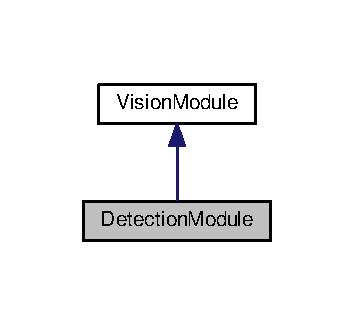
\includegraphics[width=170pt]{classDetectionModule__inherit__graph}
\end{center}
\end{figure}


Collaboration diagram for Detection\+Module\+:\nopagebreak
\begin{figure}[H]
\begin{center}
\leavevmode
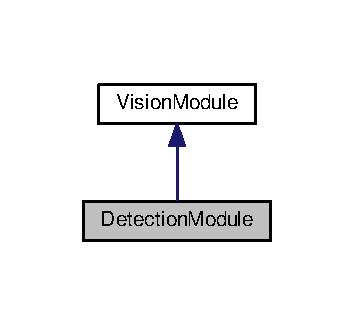
\includegraphics[width=170pt]{classDetectionModule__coll__graph}
\end{center}
\end{figure}
\subsection*{Public Member Functions}
\begin{DoxyCompactItemize}
\item 
\hyperlink{classDetectionModule_a4932f860fdbd74d8e6c05a7d8c38663b}{Detection\+Module} ()\hypertarget{classDetectionModule_a4932f860fdbd74d8e6c05a7d8c38663b}{}\label{classDetectionModule_a4932f860fdbd74d8e6c05a7d8c38663b}

\begin{DoxyCompactList}\small\item\em Constructor for class. \end{DoxyCompactList}\item 
\hyperlink{classDetectionModule_aead68009e498043dcfb41549c8bc9b12}{$\sim$\+Detection\+Module} ()\hypertarget{classDetectionModule_aead68009e498043dcfb41549c8bc9b12}{}\label{classDetectionModule_aead68009e498043dcfb41549c8bc9b12}

\begin{DoxyCompactList}\small\item\em Destrcutor for class. \end{DoxyCompactList}\item 
int \hyperlink{classDetectionModule_a19425b06ff8ab05da7baf445da26f94a}{detect\+Objects} (cv\+::\+Mat image)
\begin{DoxyCompactList}\small\item\em Function passes the processed image to the network. \end{DoxyCompactList}\item 
cv\+::\+Mat \hyperlink{classDetectionModule_a50f820e631ffbda26d20a1b2fb6b5790}{pre\+Process\+Image} (cv\+::\+Mat image, char filter\+Type)
\begin{DoxyCompactList}\small\item\em Processes the current frame (image) before passing to the detection network. \end{DoxyCompactList}\item 
cv\+::\+Mat \hyperlink{classDetectionModule_a2f4d5396fb17a484f6f9905598070e47}{post\+Process\+Image} (cv\+::\+Mat frame, int frame\+ID)
\begin{DoxyCompactList}\small\item\em Processes the current frame (image) and the obtained detection information from the detection network. \end{DoxyCompactList}\item 
void \hyperlink{classDetectionModule_ae6cbbbc1bfd1326b8ebbd83bc9e714bf}{get\+Input} ()
\begin{DoxyCompactList}\small\item\em Function to get input from user. Uses \hyperlink{classIOHandler}{I\+O\+Handler} functionality. \end{DoxyCompactList}\item 
int \hyperlink{classDetectionModule_a8d9d9c0e5b988ce56a290fa0e1fe56ae}{get\+Frame} (std\+::string file\+Path, int camera\+ID, std\+::string output\+Directory, int choice)
\begin{DoxyCompactList}\small\item\em Function to call all the other functions of the class and also the functions of class with part of relationship. \end{DoxyCompactList}\end{DoxyCompactItemize}


\subsection{Detailed Description}
Class for Implementing Human Obstacle Detection Algorithms. 

Inherits from \hyperlink{classVisionModule}{Vision\+Module} class 

\subsection{Member Function Documentation}
\index{Detection\+Module@{Detection\+Module}!detect\+Objects@{detect\+Objects}}
\index{detect\+Objects@{detect\+Objects}!Detection\+Module@{Detection\+Module}}
\subsubsection[{\texorpdfstring{detect\+Objects(cv\+::\+Mat image)}{detectObjects(cv::Mat image)}}]{\setlength{\rightskip}{0pt plus 5cm}auto Detection\+Module\+::detect\+Objects (
\begin{DoxyParamCaption}
\item[{cv\+::\+Mat}]{image}
\end{DoxyParamCaption}
)}\hypertarget{classDetectionModule_a19425b06ff8ab05da7baf445da26f94a}{}\label{classDetectionModule_a19425b06ff8ab05da7baf445da26f94a}


Function passes the processed image to the network. 

The functions takes input the processed image and then calls another function inside it to convert the image to blob


\begin{DoxyParams}{Parameters}
{\em image} & the processed image in form of the matrix \\
\hline
\end{DoxyParams}
\begin{DoxyReturn}{Returns}
Returns an int with an error code. Returns 0 if the total number of the detections is zero and 1 if not. 
\end{DoxyReturn}
\index{Detection\+Module@{Detection\+Module}!get\+Frame@{get\+Frame}}
\index{get\+Frame@{get\+Frame}!Detection\+Module@{Detection\+Module}}
\subsubsection[{\texorpdfstring{get\+Frame(std\+::string file\+Path, int camera\+I\+D, std\+::string output\+Directory, int choice)}{getFrame(std::string filePath, int cameraID, std::string outputDirectory, int choice)}}]{\setlength{\rightskip}{0pt plus 5cm}auto Detection\+Module\+::get\+Frame (
\begin{DoxyParamCaption}
\item[{std\+::string}]{file\+Path, }
\item[{int}]{camera\+ID, }
\item[{std\+::string}]{output\+Directory, }
\item[{int}]{choice}
\end{DoxyParamCaption}
)}\hypertarget{classDetectionModule_a8d9d9c0e5b988ce56a290fa0e1fe56ae}{}\label{classDetectionModule_a8d9d9c0e5b988ce56a290fa0e1fe56ae}


Function to call all the other functions of the class and also the functions of class with part of relationship. 

This function performs the fundamental role in the module. It integrates all the preprocess and postprocess of the data with the functionality of the network.


\begin{DoxyParams}{Parameters}
{\em file\+Path} & contains the path of the file to be parsed and feeded to the network. \\
\hline
{\em camera\+ID} & contains the camera\+ID if user choses camera to be the mode of input. \\
\hline
{\em output\+Directory} & path where the results need to be stored \\
\hline
{\em choice} & Choice of input format(image/video/camera) given by user\\
\hline
\end{DoxyParams}
\begin{DoxyReturn}{Returns}
0 if the data is invalid or the camera\+ID is invalid and return 1 if the module runs successfully. 
\end{DoxyReturn}
\index{Detection\+Module@{Detection\+Module}!get\+Input@{get\+Input}}
\index{get\+Input@{get\+Input}!Detection\+Module@{Detection\+Module}}
\subsubsection[{\texorpdfstring{get\+Input()}{getInput()}}]{\setlength{\rightskip}{0pt plus 5cm}auto Detection\+Module\+::get\+Input (
\begin{DoxyParamCaption}
{}
\end{DoxyParamCaption}
)}\hypertarget{classDetectionModule_ae6cbbbc1bfd1326b8ebbd83bc9e714bf}{}\label{classDetectionModule_ae6cbbbc1bfd1326b8ebbd83bc9e714bf}


Function to get input from user. Uses \hyperlink{classIOHandler}{I\+O\+Handler} functionality. 

\begin{DoxyReturn}{Returns}
void 
\end{DoxyReturn}
\index{Detection\+Module@{Detection\+Module}!post\+Process\+Image@{post\+Process\+Image}}
\index{post\+Process\+Image@{post\+Process\+Image}!Detection\+Module@{Detection\+Module}}
\subsubsection[{\texorpdfstring{post\+Process\+Image(cv\+::\+Mat frame, int frame\+I\+D)}{postProcessImage(cv::Mat frame, int frameID)}}]{\setlength{\rightskip}{0pt plus 5cm}auto Detection\+Module\+::post\+Process\+Image (
\begin{DoxyParamCaption}
\item[{cv\+::\+Mat}]{frame, }
\item[{int}]{frame\+ID}
\end{DoxyParamCaption}
)}\hypertarget{classDetectionModule_a2f4d5396fb17a484f6f9905598070e47}{}\label{classDetectionModule_a2f4d5396fb17a484f6f9905598070e47}


Processes the current frame (image) and the obtained detection information from the detection network. 

Filters obtained bounding boxes predicted from the network (using confidence threshold) and calls the function to apply N\+MS and draw the boxes on image for visualization.


\begin{DoxyParams}{Parameters}
{\em frame} & image on which the post\+Processing would occur \\
\hline
{\em frame\+ID} & ID of the frame which is parsed\\
\hline
\end{DoxyParams}
\begin{DoxyReturn}{Returns}
Image after Processing 
\end{DoxyReturn}
\index{Detection\+Module@{Detection\+Module}!pre\+Process\+Image@{pre\+Process\+Image}}
\index{pre\+Process\+Image@{pre\+Process\+Image}!Detection\+Module@{Detection\+Module}}
\subsubsection[{\texorpdfstring{pre\+Process\+Image(cv\+::\+Mat image, char filter\+Type)}{preProcessImage(cv::Mat image, char filterType)}}]{\setlength{\rightskip}{0pt plus 5cm}auto Detection\+Module\+::pre\+Process\+Image (
\begin{DoxyParamCaption}
\item[{cv\+::\+Mat}]{image, }
\item[{char}]{filter\+Type}
\end{DoxyParamCaption}
)}\hypertarget{classDetectionModule_a50f820e631ffbda26d20a1b2fb6b5790}{}\label{classDetectionModule_a50f820e631ffbda26d20a1b2fb6b5790}


Processes the current frame (image) before passing to the detection network. 

Removes noise from the image and resizes it to appropriate shape


\begin{DoxyParams}{Parameters}
{\em image} & Current frame (image) on which detection is to be done \\
\hline
{\em filter\+Type} & Type of filter to be used for removing noise\\
\hline
\end{DoxyParams}
\begin{DoxyReturn}{Returns}
Image after Processing 
\end{DoxyReturn}


The documentation for this class was generated from the following files\+:\begin{DoxyCompactItemize}
\item 
include/\hyperlink{DetectionModule_8hpp}{Detection\+Module.\+hpp}\item 
app/\hyperlink{DetectionModule_8cpp}{Detection\+Module.\+cpp}\end{DoxyCompactItemize}

\hypertarget{classIOHandler}{}\section{I\+O\+Handler Class Reference}
\label{classIOHandler}\index{I\+O\+Handler@{I\+O\+Handler}}


Class to manage the input output functionality of the module.  




{\ttfamily \#include $<$I\+O\+Handler.\+hpp$>$}

\subsection*{Public Member Functions}
\begin{DoxyCompactItemize}
\item 
\hyperlink{classIOHandler_a27272b659d19b90caa9f82d5eefb3d89}{I\+O\+Handler} ()\hypertarget{classIOHandler_a27272b659d19b90caa9f82d5eefb3d89}{}\label{classIOHandler_a27272b659d19b90caa9f82d5eefb3d89}

\begin{DoxyCompactList}\small\item\em Default constructor. \end{DoxyCompactList}\item 
\hyperlink{classIOHandler_af0e55c7ef92c62d7346883c0e66e4f1f}{I\+O\+Handler} (std\+::istream \&input, std\+::ostream \&output)
\begin{DoxyCompactList}\small\item\em Parametric constructor. \end{DoxyCompactList}\item 
\hyperlink{classIOHandler_aef78ba30518e3fa1951424ff3adb0490}{$\sim$\+I\+O\+Handler} ()\hypertarget{classIOHandler_aef78ba30518e3fa1951424ff3adb0490}{}\label{classIOHandler_aef78ba30518e3fa1951424ff3adb0490}

\begin{DoxyCompactList}\small\item\em Default Destructor. \end{DoxyCompactList}\item 
int \hyperlink{classIOHandler_a3f67a9ba2c496895443cd12af0786749}{get\+Input\+Choice} ()
\begin{DoxyCompactList}\small\item\em Takes the input from the user. \end{DoxyCompactList}\item 
std\+::string \hyperlink{classIOHandler_a0cd2ab4b1fea5696e63e626b0ade9182}{get\+Input\+File\+Path} ()
\begin{DoxyCompactList}\small\item\em Takes the input file path from the user. \end{DoxyCompactList}\item 
int \hyperlink{classIOHandler_ab032ccce83ab9fdd990dd163bc791f57}{get\+Device\+ID} ()
\begin{DoxyCompactList}\small\item\em Takes the device ID if the input is taken using camera. \end{DoxyCompactList}\item 
std\+::string \hyperlink{classIOHandler_a2bc83b86cbec3a5bea71d28e7abaa58e}{get\+Output\+File\+Path} ()
\begin{DoxyCompactList}\small\item\em Gets the path of the output directory to story detections and and text files. \end{DoxyCompactList}\item 
void \hyperlink{classIOHandler_a86d53a227457528275b8ab3bd653654f}{save\+Output} (std\+::vector$<$ std\+::vector$<$ int $>$ $>$ final\+Detections, std\+::string output\+Directory)
\begin{DoxyCompactList}\small\item\em Saves the text file in the output directory. \end{DoxyCompactList}\end{DoxyCompactItemize}


\subsection{Detailed Description}
Class to manage the input output functionality of the module. 

\subsection{Constructor \& Destructor Documentation}
\index{I\+O\+Handler@{I\+O\+Handler}!I\+O\+Handler@{I\+O\+Handler}}
\index{I\+O\+Handler@{I\+O\+Handler}!I\+O\+Handler@{I\+O\+Handler}}
\subsubsection[{\texorpdfstring{I\+O\+Handler(std\+::istream \&input, std\+::ostream \&output)}{IOHandler(std::istream &input, std::ostream &output)}}]{\setlength{\rightskip}{0pt plus 5cm}I\+O\+Handler\+::\+I\+O\+Handler (
\begin{DoxyParamCaption}
\item[{std\+::istream \&}]{input, }
\item[{std\+::ostream \&}]{output}
\end{DoxyParamCaption}
)}\hypertarget{classIOHandler_af0e55c7ef92c62d7346883c0e66e4f1f}{}\label{classIOHandler_af0e55c7ef92c62d7346883c0e66e4f1f}


Parametric constructor. 


\begin{DoxyParams}{Parameters}
{\em input} & the input entered by the user \\
\hline
{\em output} & the information to be output by the module \\
\hline
\end{DoxyParams}


\subsection{Member Function Documentation}
\index{I\+O\+Handler@{I\+O\+Handler}!get\+Device\+ID@{get\+Device\+ID}}
\index{get\+Device\+ID@{get\+Device\+ID}!I\+O\+Handler@{I\+O\+Handler}}
\subsubsection[{\texorpdfstring{get\+Device\+I\+D()}{getDeviceID()}}]{\setlength{\rightskip}{0pt plus 5cm}auto I\+O\+Handler\+::get\+Device\+ID (
\begin{DoxyParamCaption}
{}
\end{DoxyParamCaption}
)}\hypertarget{classIOHandler_ab032ccce83ab9fdd990dd163bc791f57}{}\label{classIOHandler_ab032ccce83ab9fdd990dd163bc791f57}


Takes the device ID if the input is taken using camera. 

\begin{DoxyReturn}{Returns}
the ID of the device 
\end{DoxyReturn}
\index{I\+O\+Handler@{I\+O\+Handler}!get\+Input\+Choice@{get\+Input\+Choice}}
\index{get\+Input\+Choice@{get\+Input\+Choice}!I\+O\+Handler@{I\+O\+Handler}}
\subsubsection[{\texorpdfstring{get\+Input\+Choice()}{getInputChoice()}}]{\setlength{\rightskip}{0pt plus 5cm}auto I\+O\+Handler\+::get\+Input\+Choice (
\begin{DoxyParamCaption}
{}
\end{DoxyParamCaption}
)}\hypertarget{classIOHandler_a3f67a9ba2c496895443cd12af0786749}{}\label{classIOHandler_a3f67a9ba2c496895443cd12af0786749}


Takes the input from the user. 

Takes the input of the options from the user and also checks whether the input is valid or not

\begin{DoxyReturn}{Returns}
the integer entered by the user as a choice 
\end{DoxyReturn}
Loop to enforce that user choose one of the provided options \index{I\+O\+Handler@{I\+O\+Handler}!get\+Input\+File\+Path@{get\+Input\+File\+Path}}
\index{get\+Input\+File\+Path@{get\+Input\+File\+Path}!I\+O\+Handler@{I\+O\+Handler}}
\subsubsection[{\texorpdfstring{get\+Input\+File\+Path()}{getInputFilePath()}}]{\setlength{\rightskip}{0pt plus 5cm}auto I\+O\+Handler\+::get\+Input\+File\+Path (
\begin{DoxyParamCaption}
{}
\end{DoxyParamCaption}
)}\hypertarget{classIOHandler_a0cd2ab4b1fea5696e63e626b0ade9182}{}\label{classIOHandler_a0cd2ab4b1fea5696e63e626b0ade9182}


Takes the input file path from the user. 

Also checks whether the file mentioned exists or not

\begin{DoxyReturn}{Returns}
path of the input file as entered by the user 
\end{DoxyReturn}
Loop to check that the path given by the user is correct or not \index{I\+O\+Handler@{I\+O\+Handler}!get\+Output\+File\+Path@{get\+Output\+File\+Path}}
\index{get\+Output\+File\+Path@{get\+Output\+File\+Path}!I\+O\+Handler@{I\+O\+Handler}}
\subsubsection[{\texorpdfstring{get\+Output\+File\+Path()}{getOutputFilePath()}}]{\setlength{\rightskip}{0pt plus 5cm}auto I\+O\+Handler\+::get\+Output\+File\+Path (
\begin{DoxyParamCaption}
{}
\end{DoxyParamCaption}
)}\hypertarget{classIOHandler_a2bc83b86cbec3a5bea71d28e7abaa58e}{}\label{classIOHandler_a2bc83b86cbec3a5bea71d28e7abaa58e}


Gets the path of the output directory to story detections and and text files. 

\begin{DoxyReturn}{Returns}
path of the directory where the results will be stored 
\end{DoxyReturn}
\index{I\+O\+Handler@{I\+O\+Handler}!save\+Output@{save\+Output}}
\index{save\+Output@{save\+Output}!I\+O\+Handler@{I\+O\+Handler}}
\subsubsection[{\texorpdfstring{save\+Output(std\+::vector$<$ std\+::vector$<$ int $>$ $>$ final\+Detections, std\+::string output\+Directory)}{saveOutput(std::vector< std::vector< int > > finalDetections, std::string outputDirectory)}}]{\setlength{\rightskip}{0pt plus 5cm}auto I\+O\+Handler\+::save\+Output (
\begin{DoxyParamCaption}
\item[{std\+::vector$<$ std\+::vector$<$ int $>$ $>$}]{final\+Detections, }
\item[{std\+::string}]{output\+Directory}
\end{DoxyParamCaption}
)}\hypertarget{classIOHandler_a86d53a227457528275b8ab3bd653654f}{}\label{classIOHandler_a86d53a227457528275b8ab3bd653654f}


Saves the text file in the output directory. 


\begin{DoxyParams}{Parameters}
{\em final\+Detections} & Vector of vectors to store the final detections after the complete preprocessing \\
\hline
{\em output\+Directory} & the path of the directory to store the results\\
\hline
\end{DoxyParams}
\begin{DoxyReturn}{Returns}
void 
\end{DoxyReturn}


The documentation for this class was generated from the following files\+:\begin{DoxyCompactItemize}
\item 
include/\hyperlink{IOHandler_8hpp}{I\+O\+Handler.\+hpp}\item 
app/\hyperlink{IOHandler_8cpp}{I\+O\+Handler.\+cpp}\end{DoxyCompactItemize}

\hypertarget{classNetwork}{}\section{Network Class Reference}
\label{classNetwork}\index{Network@{Network}}


Class for Implementing Neural \hyperlink{classNetwork}{Network} for Human Detection.  




{\ttfamily \#include $<$Network.\+hpp$>$}

\subsection*{Public Member Functions}
\begin{DoxyCompactItemize}
\item 
\hyperlink{classNetwork_a3cc2fb4f8fa4d507077e8da85ce5a1c8}{Network} ()\hypertarget{classNetwork_a3cc2fb4f8fa4d507077e8da85ce5a1c8}{}\label{classNetwork_a3cc2fb4f8fa4d507077e8da85ce5a1c8}

\begin{DoxyCompactList}\small\item\em Constructor for class. \end{DoxyCompactList}\item 
\hyperlink{classNetwork_a7a4e19cdb4bf0c7ecf82baa643831492}{$\sim$\+Network} ()\hypertarget{classNetwork_a7a4e19cdb4bf0c7ecf82baa643831492}{}\label{classNetwork_a7a4e19cdb4bf0c7ecf82baa643831492}

\begin{DoxyCompactList}\small\item\em Destrcutor for class. \end{DoxyCompactList}\item 
int \hyperlink{classNetwork_a45a6aa8bbd1faf0c67024d561eba0d4d}{create\+Network\+Input} (cv\+::\+Mat image)
\begin{DoxyCompactList}\small\item\em Function to convert the given image input into appropriate format for the network. \end{DoxyCompactList}\item 
std\+::vector$<$ cv\+::\+Mat $>$ \hyperlink{classNetwork_a2db1f347f5d12693f959723039bc26f4}{apply\+Y\+O\+L\+O\+Network} ()
\begin{DoxyCompactList}\small\item\em Applies the network for human detection. \end{DoxyCompactList}\end{DoxyCompactItemize}


\subsection{Detailed Description}
Class for Implementing Neural \hyperlink{classNetwork}{Network} for Human Detection. 

\subsection{Member Function Documentation}
\index{Network@{Network}!apply\+Y\+O\+L\+O\+Network@{apply\+Y\+O\+L\+O\+Network}}
\index{apply\+Y\+O\+L\+O\+Network@{apply\+Y\+O\+L\+O\+Network}!Network@{Network}}
\subsubsection[{\texorpdfstring{apply\+Y\+O\+L\+O\+Network()}{applyYOLONetwork()}}]{\setlength{\rightskip}{0pt plus 5cm}auto Network\+::apply\+Y\+O\+L\+O\+Network (
\begin{DoxyParamCaption}
{}
\end{DoxyParamCaption}
)}\hypertarget{classNetwork_a2db1f347f5d12693f959723039bc26f4}{}\label{classNetwork_a2db1f347f5d12693f959723039bc26f4}


Applies the network for human detection. 

\begin{DoxyReturn}{Returns}
Vector of matrices(and a Image) containing detection information 
\end{DoxyReturn}
\index{Network@{Network}!create\+Network\+Input@{create\+Network\+Input}}
\index{create\+Network\+Input@{create\+Network\+Input}!Network@{Network}}
\subsubsection[{\texorpdfstring{create\+Network\+Input(cv\+::\+Mat image)}{createNetworkInput(cv::Mat image)}}]{\setlength{\rightskip}{0pt plus 5cm}auto Network\+::create\+Network\+Input (
\begin{DoxyParamCaption}
\item[{cv\+::\+Mat}]{image}
\end{DoxyParamCaption}
)}\hypertarget{classNetwork_a45a6aa8bbd1faf0c67024d561eba0d4d}{}\label{classNetwork_a45a6aa8bbd1faf0c67024d561eba0d4d}


Function to convert the given image input into appropriate format for the network. 


\begin{DoxyParams}{Parameters}
{\em image} & Input image on which the detection is to be performed\\
\hline
\end{DoxyParams}
\begin{DoxyReturn}{Returns}
Image in appropriate format for the network 
\end{DoxyReturn}


The documentation for this class was generated from the following files\+:\begin{DoxyCompactItemize}
\item 
include/\hyperlink{Network_8hpp}{Network.\+hpp}\item 
app/\hyperlink{Network_8cpp}{Network.\+cpp}\end{DoxyCompactItemize}

\hypertarget{classTransformation}{}\section{Transformation Class Reference}
\label{classTransformation}\index{Transformation@{Transformation}}


Class for implementing Frame transformations.  




{\ttfamily \#include $<$Transformation.\+hpp$>$}

\subsection*{Public Member Functions}
\begin{DoxyCompactItemize}
\item 
\hyperlink{classTransformation_a40ab64d41c752804740e972ef5f2479f}{Transformation} ()
\begin{DoxyCompactList}\small\item\em Constructor for class. \end{DoxyCompactList}\item 
\hyperlink{classTransformation_a919fd564686f686ff8060fc85d14e3f7}{Transformation} (cv\+::\+Mat base, cv\+::\+Mat end)
\begin{DoxyCompactList}\small\item\em Constructor for class with base and end frame input. \end{DoxyCompactList}\item 
\hyperlink{classTransformation_ade11a9f133b2acd81ae9383187cc255e}{$\sim$\+Transformation} ()\hypertarget{classTransformation_ade11a9f133b2acd81ae9383187cc255e}{}\label{classTransformation_ade11a9f133b2acd81ae9383187cc255e}

\begin{DoxyCompactList}\small\item\em Destrcutor for class. \end{DoxyCompactList}\item 
cv\+::\+Mat \hyperlink{classTransformation_afcce8d7bce0b4760e90b2c9a4f33778b}{base\+To\+End} (cv\+::\+Mat vec)
\begin{DoxyCompactList}\small\item\em Function to convert vector in base frame to end frame. \end{DoxyCompactList}\item 
cv\+::\+Mat \hyperlink{classTransformation_ae06ef579b76564a33e5db35f7d617161}{end\+To\+Base} (cv\+::\+Mat vec)
\begin{DoxyCompactList}\small\item\em Function to convert vector in end frame to base frame. \end{DoxyCompactList}\item 
cv\+::\+Mat \hyperlink{classTransformation_a8a7c06d699c43a020069098aac504e27}{image\+To\+Camera} (cv\+::\+Mat intrinsic, cv\+::\+Mat vec\+Image2d)
\begin{DoxyCompactList}\small\item\em Function to convert image coordinates to Camera coordinates. \end{DoxyCompactList}\item 
cv\+::\+Mat \hyperlink{classTransformation_a9e7afec78535b499d99c8d55e08f91f1}{camera\+To\+Image} (cv\+::\+Mat intrinsic, cv\+::\+Mat vec\+Camera4d)
\begin{DoxyCompactList}\small\item\em Function to convert Camera coordinates to image coordinates. \end{DoxyCompactList}\item 
cv\+::\+Mat \hyperlink{classTransformation_a0536abd126af1fcffd0b7644ebf0b108}{get\+Base\+Frame} ()
\begin{DoxyCompactList}\small\item\em Function to return base frame. \end{DoxyCompactList}\item 
cv\+::\+Mat \hyperlink{classTransformation_aea3e04cbe0289fcd34b51c6541a23242}{get\+End\+Frame} ()
\begin{DoxyCompactList}\small\item\em Function to return end frame. \end{DoxyCompactList}\end{DoxyCompactItemize}


\subsection{Detailed Description}
Class for implementing Frame transformations. 

\subsection{Constructor \& Destructor Documentation}
\index{Transformation@{Transformation}!Transformation@{Transformation}}
\index{Transformation@{Transformation}!Transformation@{Transformation}}
\subsubsection[{\texorpdfstring{Transformation()}{Transformation()}}]{\setlength{\rightskip}{0pt plus 5cm}Transformation\+::\+Transformation (
\begin{DoxyParamCaption}
{}
\end{DoxyParamCaption}
)}\hypertarget{classTransformation_a40ab64d41c752804740e972ef5f2479f}{}\label{classTransformation_a40ab64d41c752804740e972ef5f2479f}


Constructor for class. 

Initializes base and end frames as identity matrices \index{Transformation@{Transformation}!Transformation@{Transformation}}
\index{Transformation@{Transformation}!Transformation@{Transformation}}
\subsubsection[{\texorpdfstring{Transformation(cv\+::\+Mat base, cv\+::\+Mat end)}{Transformation(cv::Mat base, cv::Mat end)}}]{\setlength{\rightskip}{0pt plus 5cm}Transformation\+::\+Transformation (
\begin{DoxyParamCaption}
\item[{cv\+::\+Mat}]{base, }
\item[{cv\+::\+Mat}]{end}
\end{DoxyParamCaption}
)}\hypertarget{classTransformation_a919fd564686f686ff8060fc85d14e3f7}{}\label{classTransformation_a919fd564686f686ff8060fc85d14e3f7}


Constructor for class with base and end frame input. 


\begin{DoxyParams}{Parameters}
{\em base} & Base Frame \\
\hline
{\em end} & End effector Frame \\
\hline
\end{DoxyParams}


\subsection{Member Function Documentation}
\index{Transformation@{Transformation}!base\+To\+End@{base\+To\+End}}
\index{base\+To\+End@{base\+To\+End}!Transformation@{Transformation}}
\subsubsection[{\texorpdfstring{base\+To\+End(cv\+::\+Mat vec)}{baseToEnd(cv::Mat vec)}}]{\setlength{\rightskip}{0pt plus 5cm}auto Transformation\+::base\+To\+End (
\begin{DoxyParamCaption}
\item[{cv\+::\+Mat}]{vec}
\end{DoxyParamCaption}
)}\hypertarget{classTransformation_afcce8d7bce0b4760e90b2c9a4f33778b}{}\label{classTransformation_afcce8d7bce0b4760e90b2c9a4f33778b}


Function to convert vector in base frame to end frame. 


\begin{DoxyParams}{Parameters}
{\em vec} & Vector in base frame coordinates\\
\hline
\end{DoxyParams}
\begin{DoxyReturn}{Returns}
Vector in end frame coordinates 
\end{DoxyReturn}
\index{Transformation@{Transformation}!camera\+To\+Image@{camera\+To\+Image}}
\index{camera\+To\+Image@{camera\+To\+Image}!Transformation@{Transformation}}
\subsubsection[{\texorpdfstring{camera\+To\+Image(cv\+::\+Mat intrinsic, cv\+::\+Mat vec\+Camera4d)}{cameraToImage(cv::Mat intrinsic, cv::Mat vecCamera4d)}}]{\setlength{\rightskip}{0pt plus 5cm}auto Transformation\+::camera\+To\+Image (
\begin{DoxyParamCaption}
\item[{cv\+::\+Mat}]{intrinsic, }
\item[{cv\+::\+Mat}]{vec\+Camera4d}
\end{DoxyParamCaption}
)}\hypertarget{classTransformation_a9e7afec78535b499d99c8d55e08f91f1}{}\label{classTransformation_a9e7afec78535b499d99c8d55e08f91f1}


Function to convert Camera coordinates to image coordinates. 


\begin{DoxyParams}{Parameters}
{\em vec\+Camera4d} & Vector of camera coordinates \\
\hline
{\em intrinsic} & Intrinsic matric of the camera\\
\hline
\end{DoxyParams}
\begin{DoxyReturn}{Returns}
Vector in image coordinates
\end{DoxyReturn}

\begin{DoxyParams}{Parameters}
{\em vec} & Vector in end frame coordinates\\
\hline
\end{DoxyParams}
\begin{DoxyReturn}{Returns}
Vector in base frame coordinates 
\end{DoxyReturn}
\index{Transformation@{Transformation}!end\+To\+Base@{end\+To\+Base}}
\index{end\+To\+Base@{end\+To\+Base}!Transformation@{Transformation}}
\subsubsection[{\texorpdfstring{end\+To\+Base(cv\+::\+Mat vec)}{endToBase(cv::Mat vec)}}]{\setlength{\rightskip}{0pt plus 5cm}auto Transformation\+::end\+To\+Base (
\begin{DoxyParamCaption}
\item[{cv\+::\+Mat}]{vec}
\end{DoxyParamCaption}
)}\hypertarget{classTransformation_ae06ef579b76564a33e5db35f7d617161}{}\label{classTransformation_ae06ef579b76564a33e5db35f7d617161}


Function to convert vector in end frame to base frame. 


\begin{DoxyParams}{Parameters}
{\em vec} & Vector in end frame coordinates\\
\hline
\end{DoxyParams}
\begin{DoxyReturn}{Returns}
Vector in base frame coordinates 
\end{DoxyReturn}
\index{Transformation@{Transformation}!get\+Base\+Frame@{get\+Base\+Frame}}
\index{get\+Base\+Frame@{get\+Base\+Frame}!Transformation@{Transformation}}
\subsubsection[{\texorpdfstring{get\+Base\+Frame()}{getBaseFrame()}}]{\setlength{\rightskip}{0pt plus 5cm}auto Transformation\+::get\+Base\+Frame (
\begin{DoxyParamCaption}
{}
\end{DoxyParamCaption}
)}\hypertarget{classTransformation_a0536abd126af1fcffd0b7644ebf0b108}{}\label{classTransformation_a0536abd126af1fcffd0b7644ebf0b108}


Function to return base frame. 

\begin{DoxyReturn}{Returns}
Base frame 
\end{DoxyReturn}
\index{Transformation@{Transformation}!get\+End\+Frame@{get\+End\+Frame}}
\index{get\+End\+Frame@{get\+End\+Frame}!Transformation@{Transformation}}
\subsubsection[{\texorpdfstring{get\+End\+Frame()}{getEndFrame()}}]{\setlength{\rightskip}{0pt plus 5cm}auto Transformation\+::get\+End\+Frame (
\begin{DoxyParamCaption}
{}
\end{DoxyParamCaption}
)}\hypertarget{classTransformation_aea3e04cbe0289fcd34b51c6541a23242}{}\label{classTransformation_aea3e04cbe0289fcd34b51c6541a23242}


Function to return end frame. 

\begin{DoxyReturn}{Returns}
End frame 
\end{DoxyReturn}
\index{Transformation@{Transformation}!image\+To\+Camera@{image\+To\+Camera}}
\index{image\+To\+Camera@{image\+To\+Camera}!Transformation@{Transformation}}
\subsubsection[{\texorpdfstring{image\+To\+Camera(cv\+::\+Mat intrinsic, cv\+::\+Mat vec\+Image2d)}{imageToCamera(cv::Mat intrinsic, cv::Mat vecImage2d)}}]{\setlength{\rightskip}{0pt plus 5cm}auto Transformation\+::image\+To\+Camera (
\begin{DoxyParamCaption}
\item[{cv\+::\+Mat}]{intrinsic, }
\item[{cv\+::\+Mat}]{vec\+Image2d}
\end{DoxyParamCaption}
)}\hypertarget{classTransformation_a8a7c06d699c43a020069098aac504e27}{}\label{classTransformation_a8a7c06d699c43a020069098aac504e27}


Function to convert image coordinates to Camera coordinates. 


\begin{DoxyParams}{Parameters}
{\em vec\+Image2d} & Vector in image coordinates \\
\hline
{\em intrinsic} & Intrinsic matric of the camera\\
\hline
\end{DoxyParams}
\begin{DoxyReturn}{Returns}
Vector in camera frame coordinates
\end{DoxyReturn}

\begin{DoxyParams}{Parameters}
{\em vec} & Vector in end frame coordinates\\
\hline
\end{DoxyParams}
\begin{DoxyReturn}{Returns}
Vector in base frame coordinates 
\end{DoxyReturn}


The documentation for this class was generated from the following files\+:\begin{DoxyCompactItemize}
\item 
include/\hyperlink{Transformation_8hpp}{Transformation.\+hpp}\item 
app/\hyperlink{Transformation_8cpp}{Transformation.\+cpp}\end{DoxyCompactItemize}

\hypertarget{classVisionModule}{}\section{Vision\+Module Class Reference}
\label{classVisionModule}\index{Vision\+Module@{Vision\+Module}}


Class for Vision based functionality.  




{\ttfamily \#include $<$Vision\+Module.\+hpp$>$}



Inheritance diagram for Vision\+Module\+:\nopagebreak
\begin{figure}[H]
\begin{center}
\leavevmode
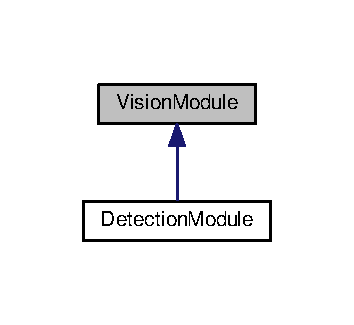
\includegraphics[width=170pt]{classVisionModule__inherit__graph}
\end{center}
\end{figure}
\subsection*{Public Member Functions}
\begin{DoxyCompactItemize}
\item 
\hyperlink{classVisionModule_a08440f0aeb474f1927b98e01953f47b0}{Vision\+Module} ()\hypertarget{classVisionModule_a08440f0aeb474f1927b98e01953f47b0}{}\label{classVisionModule_a08440f0aeb474f1927b98e01953f47b0}

\begin{DoxyCompactList}\small\item\em Constructor for class. \end{DoxyCompactList}\item 
virtual \hyperlink{classVisionModule_a820fbd8149b606d24135e2738beb50ec}{$\sim$\+Vision\+Module} ()\hypertarget{classVisionModule_a820fbd8149b606d24135e2738beb50ec}{}\label{classVisionModule_a820fbd8149b606d24135e2738beb50ec}

\begin{DoxyCompactList}\small\item\em Destrcutor for class. \end{DoxyCompactList}\item 
cv\+::\+Mat \hyperlink{classVisionModule_a03604428a8b644291e24046b306250a3}{apply\+Gaussian\+Filter} (cv\+::\+Mat image, cv\+::\+Size kernel\+Dim, float sigma)
\begin{DoxyCompactList}\small\item\em Applies Gaussian Filter to given image. \end{DoxyCompactList}\item 
cv\+::\+Mat \hyperlink{classVisionModule_af8f8e435bac0d2db615b169de62567b9}{apply\+Filter} (cv\+::\+Mat image, cv\+::\+Size kernel\+Dim)
\begin{DoxyCompactList}\small\item\em Applies Mean Filter to given image. \end{DoxyCompactList}\item 
cv\+::\+Mat \hyperlink{classVisionModule_ac80542fc84b24a098d8334f924e36971}{apply\+Median\+Filter} (cv\+::\+Mat image, int kernel\+Dim)
\begin{DoxyCompactList}\small\item\em Applies Median Filter to given image. \end{DoxyCompactList}\item 
cv\+::\+Mat \hyperlink{classVisionModule_af6d95de1a23cb8d6ec6f646d1906fd63}{reshape} (cv\+::\+Mat image, cv\+::\+Size dim)
\begin{DoxyCompactList}\small\item\em Reshapes given image to given dimension. \end{DoxyCompactList}\item 
std\+::vector$<$ std\+::vector$<$ int $>$ $>$ \hyperlink{classVisionModule_a5fb286b3086a7235fda74ab7258bb227}{non\+Maximal\+Suppression} (cv\+::\+Mat \&frame, std\+::vector$<$ cv\+::\+Rect $>$ \&predicted\+Boxes, std\+::vector$<$ float $>$ confidence\+Scores, std\+::vector$<$ int $>$ class\+Ids, int frame\+ID)
\begin{DoxyCompactList}\small\item\em Applies Non Maximal Suppression Algorithm. \end{DoxyCompactList}\end{DoxyCompactItemize}


\subsection{Detailed Description}
Class for Vision based functionality. 

\subsection{Member Function Documentation}
\index{Vision\+Module@{Vision\+Module}!apply\+Filter@{apply\+Filter}}
\index{apply\+Filter@{apply\+Filter}!Vision\+Module@{Vision\+Module}}
\subsubsection[{\texorpdfstring{apply\+Filter(cv\+::\+Mat image, cv\+::\+Size kernel\+Dim)}{applyFilter(cv::Mat image, cv::Size kernelDim)}}]{\setlength{\rightskip}{0pt plus 5cm}auto Vision\+Module\+::apply\+Filter (
\begin{DoxyParamCaption}
\item[{cv\+::\+Mat}]{image, }
\item[{cv\+::\+Size}]{kernel\+Dim}
\end{DoxyParamCaption}
)}\hypertarget{classVisionModule_af8f8e435bac0d2db615b169de62567b9}{}\label{classVisionModule_af8f8e435bac0d2db615b169de62567b9}


Applies Mean Filter to given image. 


\begin{DoxyParams}{Parameters}
{\em image} & Image on which the filter will be applied \\
\hline
{\em kernel\+Dim} & Size of kernel matrix\\
\hline
\end{DoxyParams}
\begin{DoxyReturn}{Returns}
Image after applying filter 
\end{DoxyReturn}
\index{Vision\+Module@{Vision\+Module}!apply\+Gaussian\+Filter@{apply\+Gaussian\+Filter}}
\index{apply\+Gaussian\+Filter@{apply\+Gaussian\+Filter}!Vision\+Module@{Vision\+Module}}
\subsubsection[{\texorpdfstring{apply\+Gaussian\+Filter(cv\+::\+Mat image, cv\+::\+Size kernel\+Dim, float sigma)}{applyGaussianFilter(cv::Mat image, cv::Size kernelDim, float sigma)}}]{\setlength{\rightskip}{0pt plus 5cm}auto Vision\+Module\+::apply\+Gaussian\+Filter (
\begin{DoxyParamCaption}
\item[{cv\+::\+Mat}]{image, }
\item[{cv\+::\+Size}]{kernel\+Dim, }
\item[{float}]{sigma}
\end{DoxyParamCaption}
)}\hypertarget{classVisionModule_a03604428a8b644291e24046b306250a3}{}\label{classVisionModule_a03604428a8b644291e24046b306250a3}


Applies Gaussian Filter to given image. 

The kernel is assumed to be a square matrix with equal sigma in both x and y directions


\begin{DoxyParams}{Parameters}
{\em image} & Image on which the filter will be applied \\
\hline
{\em kernel\+Dim} & Size of kernel matrix \\
\hline
{\em sigma} & Standard deviation for the Gaussian kernel\\
\hline
\end{DoxyParams}
\begin{DoxyReturn}{Returns}
Image after applying filter 
\end{DoxyReturn}
\index{Vision\+Module@{Vision\+Module}!apply\+Median\+Filter@{apply\+Median\+Filter}}
\index{apply\+Median\+Filter@{apply\+Median\+Filter}!Vision\+Module@{Vision\+Module}}
\subsubsection[{\texorpdfstring{apply\+Median\+Filter(cv\+::\+Mat image, int kernel\+Dim)}{applyMedianFilter(cv::Mat image, int kernelDim)}}]{\setlength{\rightskip}{0pt plus 5cm}auto Vision\+Module\+::apply\+Median\+Filter (
\begin{DoxyParamCaption}
\item[{cv\+::\+Mat}]{image, }
\item[{int}]{kernel\+Dim}
\end{DoxyParamCaption}
)}\hypertarget{classVisionModule_ac80542fc84b24a098d8334f924e36971}{}\label{classVisionModule_ac80542fc84b24a098d8334f924e36971}


Applies Median Filter to given image. 


\begin{DoxyParams}{Parameters}
{\em image} & Image on which the filter will be applied \\
\hline
{\em kernel\+Dim} & Size of kernel matrix\\
\hline
\end{DoxyParams}
\begin{DoxyReturn}{Returns}
Image after applying filter 
\end{DoxyReturn}
\index{Vision\+Module@{Vision\+Module}!non\+Maximal\+Suppression@{non\+Maximal\+Suppression}}
\index{non\+Maximal\+Suppression@{non\+Maximal\+Suppression}!Vision\+Module@{Vision\+Module}}
\subsubsection[{\texorpdfstring{non\+Maximal\+Suppression(cv\+::\+Mat \&frame, std\+::vector$<$ cv\+::\+Rect $>$ \&predicted\+Boxes, std\+::vector$<$ float $>$ confidence\+Scores, std\+::vector$<$ int $>$ class\+Ids, int frame\+I\+D)}{nonMaximalSuppression(cv::Mat &frame, std::vector< cv::Rect > &predictedBoxes, std::vector< float > confidenceScores, std::vector< int > classIds, int frameID)}}]{\setlength{\rightskip}{0pt plus 5cm}std\+::vector$<$ std\+::vector$<$ int $>$ $>$ Vision\+Module\+::non\+Maximal\+Suppression (
\begin{DoxyParamCaption}
\item[{cv\+::\+Mat \&}]{frame, }
\item[{std\+::vector$<$ cv\+::\+Rect $>$ \&}]{predicted\+Boxes, }
\item[{std\+::vector$<$ float $>$}]{confidence\+Scores, }
\item[{std\+::vector$<$ int $>$}]{class\+Ids, }
\item[{int}]{frame\+ID}
\end{DoxyParamCaption}
)}\hypertarget{classVisionModule_a5fb286b3086a7235fda74ab7258bb227}{}\label{classVisionModule_a5fb286b3086a7235fda74ab7258bb227}


Applies Non Maximal Suppression Algorithm. 

Given a set of bounding boxes of detected objects in an image, the algorithm removes overlapping boxes that may be enclosing the same object. The same function also draws the bounding boxes on the passed image.


\begin{DoxyParams}{Parameters}
{\em image} & Image on which the objects have been detected \\
\hline
{\em predicted\+Boxes} & Vector owith data type cv\+::rect, contains information of all the bounding boxes detected. In order, the information comprises of upper left and bottom right points corners of the box. \\
\hline
{\em confidence\+Scores} & Vector contains the confidence scores of all the boxes above threshold. \\
\hline
{\em class\+Ids} & vector that contain the class\+Ids of all the detections. \\
\hline
{\em frame\+ID} & denotes the frame number associated with the image.\\
\hline
\end{DoxyParams}
\begin{DoxyReturn}{Returns}
Modified Vector of bounding box information 
\end{DoxyReturn}
\index{Vision\+Module@{Vision\+Module}!reshape@{reshape}}
\index{reshape@{reshape}!Vision\+Module@{Vision\+Module}}
\subsubsection[{\texorpdfstring{reshape(cv\+::\+Mat image, cv\+::\+Size dim)}{reshape(cv::Mat image, cv::Size dim)}}]{\setlength{\rightskip}{0pt plus 5cm}auto Vision\+Module\+::reshape (
\begin{DoxyParamCaption}
\item[{cv\+::\+Mat}]{image, }
\item[{cv\+::\+Size}]{dim}
\end{DoxyParamCaption}
)}\hypertarget{classVisionModule_af6d95de1a23cb8d6ec6f646d1906fd63}{}\label{classVisionModule_af6d95de1a23cb8d6ec6f646d1906fd63}


Reshapes given image to given dimension. 


\begin{DoxyParams}{Parameters}
{\em image} & Image to be reshaped \\
\hline
{\em shape} & Pair of ints giving the Dimension the image has to be rehsaped to\\
\hline
\end{DoxyParams}
\begin{DoxyReturn}{Returns}
Image after reshaping it 
\end{DoxyReturn}


The documentation for this class was generated from the following files\+:\begin{DoxyCompactItemize}
\item 
include/\hyperlink{VisionModule_8hpp}{Vision\+Module.\+hpp}\item 
app/\hyperlink{VisionModule_8cpp}{Vision\+Module.\+cpp}\end{DoxyCompactItemize}

\chapter{File Documentation}
\hypertarget{DetectionModule_8cpp}{}\section{app/\+Detection\+Module.cpp File Reference}
\label{DetectionModule_8cpp}\index{app/\+Detection\+Module.\+cpp@{app/\+Detection\+Module.\+cpp}}


Definition for \hyperlink{classDetectionModule}{Detection\+Module} class.  


{\ttfamily \#include $<$iostream$>$}\\*
{\ttfamily \#include \char`\"{}Detection\+Module.\+hpp\char`\"{}}\\*
Include dependency graph for Detection\+Module.\+cpp\+:
\nopagebreak
\begin{figure}[H]
\begin{center}
\leavevmode
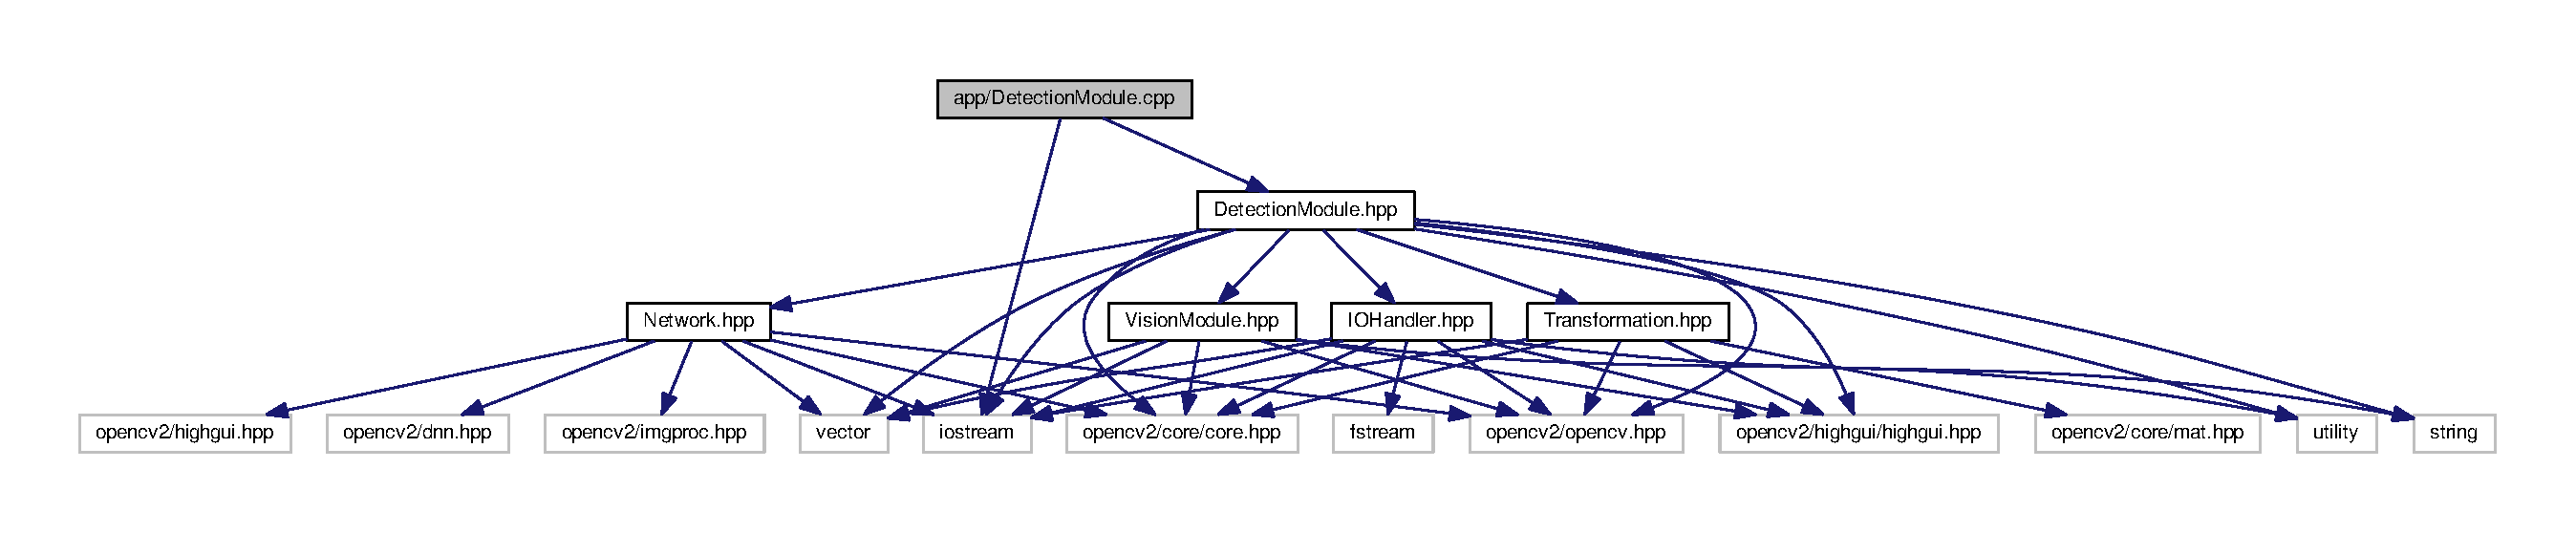
\includegraphics[width=350pt]{DetectionModule_8cpp__incl}
\end{center}
\end{figure}


\subsection{Detailed Description}
Definition for \hyperlink{classDetectionModule}{Detection\+Module} class. 

\begin{DoxyAuthor}{Author}
Rohan Singh 

Arjun Gupta 
\end{DoxyAuthor}
\begin{DoxyCopyright}{Copyright}
M\+IT License (c) 2019 Rohan Singh, Arjun Gupta 
\end{DoxyCopyright}

\hypertarget{IOHandler_8cpp}{}\section{app/\+I\+O\+Handler.cpp File Reference}
\label{IOHandler_8cpp}\index{app/\+I\+O\+Handler.\+cpp@{app/\+I\+O\+Handler.\+cpp}}


Definition for \hyperlink{classIOHandler}{I\+O\+Handler} class.  


{\ttfamily \#include $<$iostream$>$}\\*
{\ttfamily \#include \char`\"{}I\+O\+Handler.\+hpp\char`\"{}}\\*
Include dependency graph for I\+O\+Handler.\+cpp\+:
\nopagebreak
\begin{figure}[H]
\begin{center}
\leavevmode
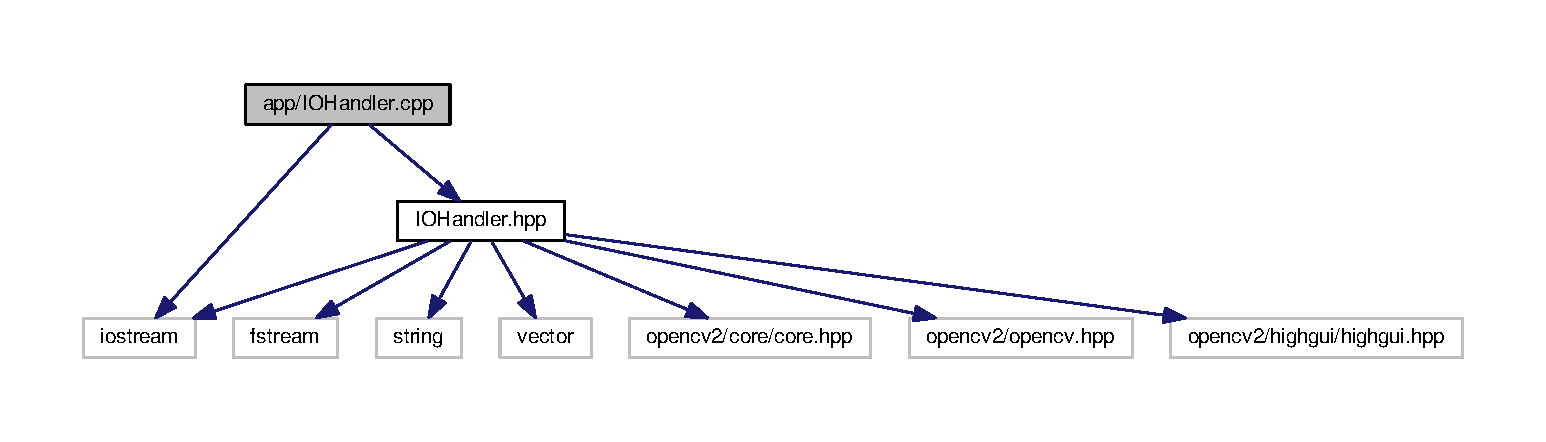
\includegraphics[width=350pt]{IOHandler_8cpp__incl}
\end{center}
\end{figure}


\subsection{Detailed Description}
Definition for \hyperlink{classIOHandler}{I\+O\+Handler} class. 

\begin{DoxyAuthor}{Author}
Rohan Singh 

Arjun Gupta 
\end{DoxyAuthor}
\begin{DoxyCopyright}{Copyright}
M\+IT License (c) 2019 Rohan Singh, Arjun Gupta 
\end{DoxyCopyright}

\hypertarget{Network_8cpp}{}\section{app/\+Network.cpp File Reference}
\label{Network_8cpp}\index{app/\+Network.\+cpp@{app/\+Network.\+cpp}}


Definition for \hyperlink{classNetwork}{Network} class.  


{\ttfamily \#include $<$iostream$>$}\\*
{\ttfamily \#include \char`\"{}../include/\+Network.\+hpp\char`\"{}}\\*
Include dependency graph for Network.\+cpp\+:\nopagebreak
\begin{figure}[H]
\begin{center}
\leavevmode
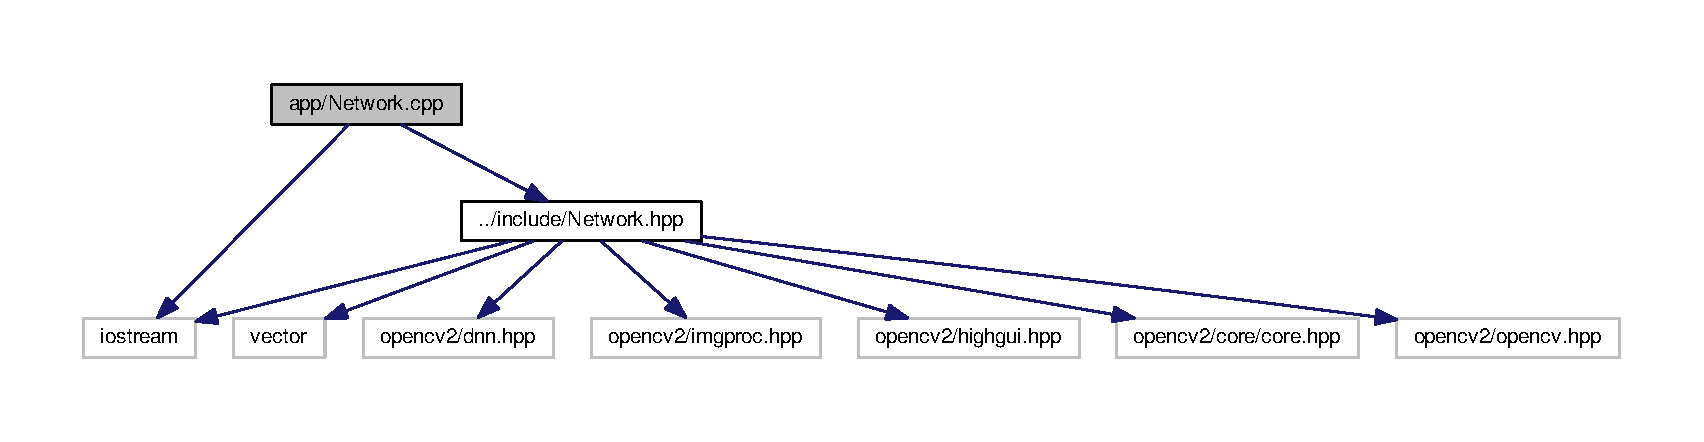
\includegraphics[width=350pt]{Network_8cpp__incl}
\end{center}
\end{figure}


\subsection{Detailed Description}
Definition for \hyperlink{classNetwork}{Network} class. 

\begin{DoxyAuthor}{Author}
Rohan Singh 

Arjun Gupta 
\end{DoxyAuthor}
\begin{DoxyCopyright}{Copyright}
M\+IT License (c) 2019 Rohan Singh, Arjun Gupta 
\end{DoxyCopyright}

\hypertarget{Transformation_8cpp}{}\section{app/\+Transformation.cpp File Reference}
\label{Transformation_8cpp}\index{app/\+Transformation.\+cpp@{app/\+Transformation.\+cpp}}


Definition for \hyperlink{classTransformation}{Transformation} class.  


{\ttfamily \#include $<$iostream$>$}\\*
{\ttfamily \#include \char`\"{}Transformation.\+hpp\char`\"{}}\\*
Include dependency graph for Transformation.\+cpp\+:\nopagebreak
\begin{figure}[H]
\begin{center}
\leavevmode
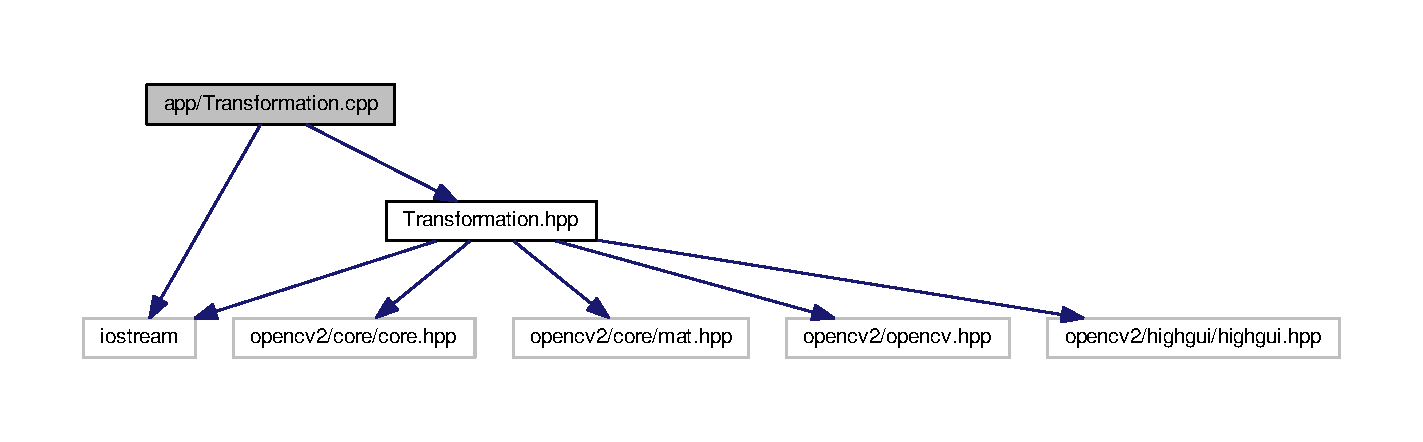
\includegraphics[width=350pt]{Transformation_8cpp__incl}
\end{center}
\end{figure}


\subsection{Detailed Description}
Definition for \hyperlink{classTransformation}{Transformation} class. 

\begin{DoxyAuthor}{Author}
Rohan Singh 

Arjun Gupta 
\end{DoxyAuthor}
\begin{DoxyCopyright}{Copyright}
M\+IT License (c) 2019 Rohan Singh, Arjun Gupta 
\end{DoxyCopyright}

\hypertarget{VisionModule_8cpp}{}\section{app/\+Vision\+Module.cpp File Reference}
\label{VisionModule_8cpp}\index{app/\+Vision\+Module.\+cpp@{app/\+Vision\+Module.\+cpp}}


Definition for \hyperlink{classVisionModule}{Vision\+Module} class.  


{\ttfamily \#include $<$iostream$>$}\\*
{\ttfamily \#include \char`\"{}Vision\+Module.\+hpp\char`\"{}}\\*
Include dependency graph for Vision\+Module.\+cpp\+:\nopagebreak
\begin{figure}[H]
\begin{center}
\leavevmode
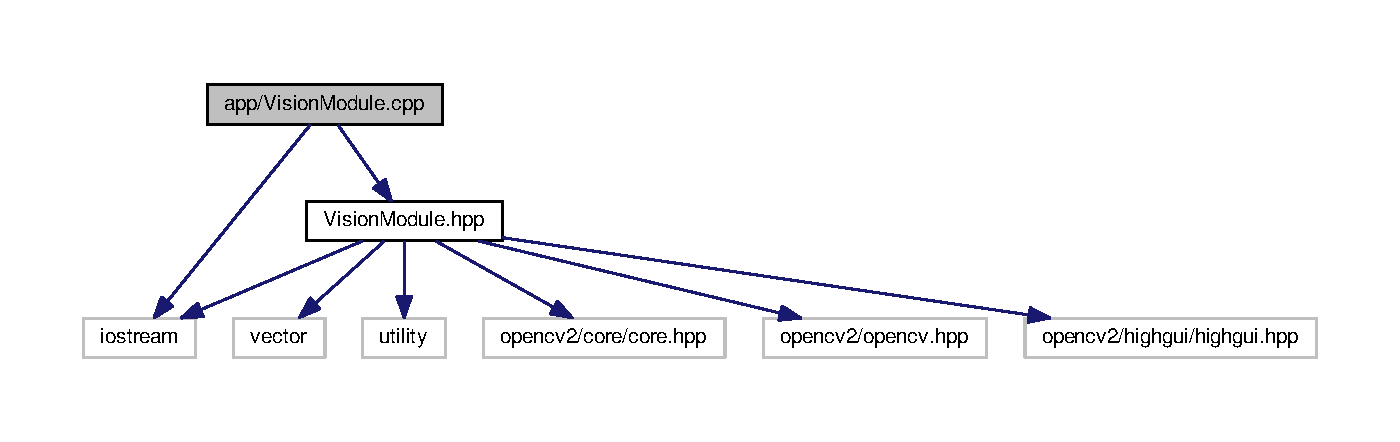
\includegraphics[width=350pt]{VisionModule_8cpp__incl}
\end{center}
\end{figure}


\subsection{Detailed Description}
Definition for \hyperlink{classVisionModule}{Vision\+Module} class. 

\begin{DoxyAuthor}{Author}
Rohan Singh 

Arjun Gupta 
\end{DoxyAuthor}
\begin{DoxyCopyright}{Copyright}
M\+IT License (c) 2019 Rohan Singh, Arjun Gupta 
\end{DoxyCopyright}

\hypertarget{DetectionModule_8hpp}{}\section{include/\+Detection\+Module.hpp File Reference}
\label{DetectionModule_8hpp}\index{include/\+Detection\+Module.\+hpp@{include/\+Detection\+Module.\+hpp}}


Declares \hyperlink{classDetectionModule}{Detection\+Module} child class inheriting from \hyperlink{classVisionModule}{Vision\+Module}.  


{\ttfamily \#include $<$iostream$>$}\\*
{\ttfamily \#include $<$vector$>$}\\*
{\ttfamily \#include $<$utility$>$}\\*
{\ttfamily \#include $<$string$>$}\\*
{\ttfamily \#include $<$opencv2/core/core.\+hpp$>$}\\*
{\ttfamily \#include $<$opencv2/opencv.\+hpp$>$}\\*
{\ttfamily \#include $<$opencv2/highgui/highgui.\+hpp$>$}\\*
{\ttfamily \#include \char`\"{}Vision\+Module.\+hpp\char`\"{}}\\*
{\ttfamily \#include \char`\"{}I\+O\+Handler.\+hpp\char`\"{}}\\*
{\ttfamily \#include \char`\"{}Network.\+hpp\char`\"{}}\\*
{\ttfamily \#include \char`\"{}Transformation.\+hpp\char`\"{}}\\*
Include dependency graph for Detection\+Module.\+hpp\+:
\nopagebreak
\begin{figure}[H]
\begin{center}
\leavevmode
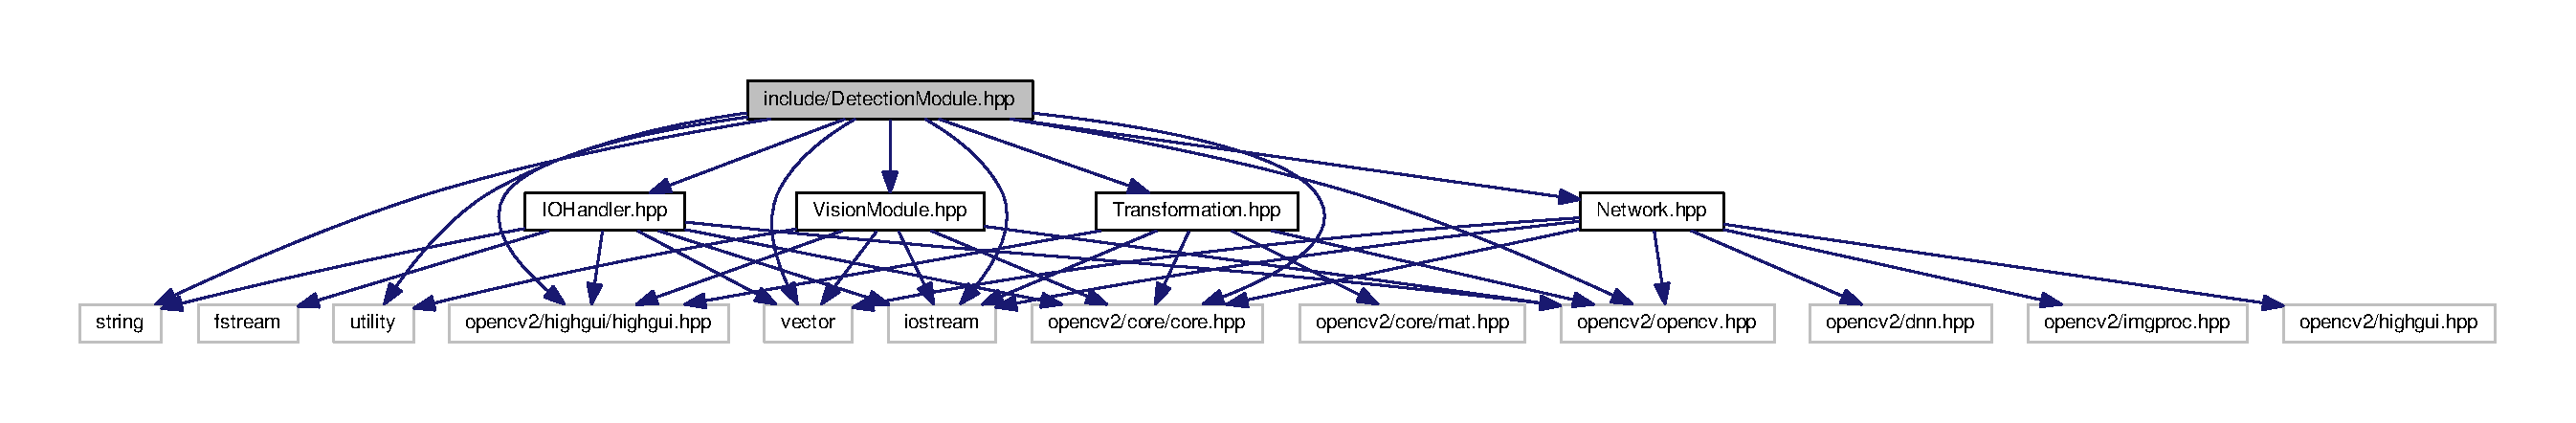
\includegraphics[width=350pt]{DetectionModule_8hpp__incl}
\end{center}
\end{figure}
This graph shows which files directly or indirectly include this file\+:\nopagebreak
\begin{figure}[H]
\begin{center}
\leavevmode
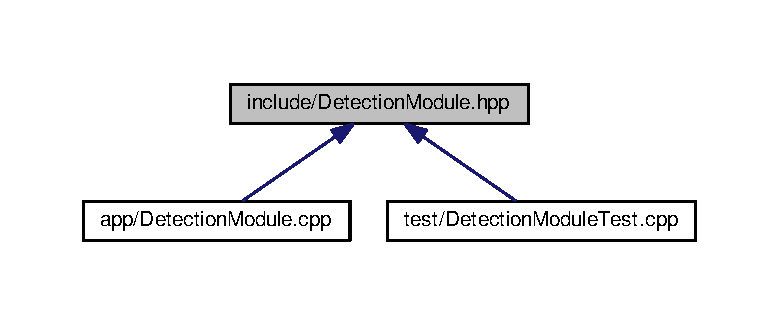
\includegraphics[width=350pt]{DetectionModule_8hpp__dep__incl}
\end{center}
\end{figure}
\subsection*{Classes}
\begin{DoxyCompactItemize}
\item 
class \hyperlink{classDetectionModule}{Detection\+Module}
\begin{DoxyCompactList}\small\item\em Class for Implementing Human Obstacle Detection Algorithms. \end{DoxyCompactList}\end{DoxyCompactItemize}


\subsection{Detailed Description}
Declares \hyperlink{classDetectionModule}{Detection\+Module} child class inheriting from \hyperlink{classVisionModule}{Vision\+Module}. 

\begin{DoxyAuthor}{Author}
Rohan Singh 

Arjun Gupta 
\end{DoxyAuthor}
\begin{DoxyCopyright}{Copyright}
M\+IT License (c) 2019 Rohan Singh, Arjun Gupta 
\end{DoxyCopyright}

\hypertarget{IOHandler_8hpp}{}\section{include/\+I\+O\+Handler.hpp File Reference}
\label{IOHandler_8hpp}\index{include/\+I\+O\+Handler.\+hpp@{include/\+I\+O\+Handler.\+hpp}}


Declares \hyperlink{classIOHandler}{I\+O\+Handler} class.  


{\ttfamily \#include $<$iostream$>$}\\*
{\ttfamily \#include $<$fstream$>$}\\*
{\ttfamily \#include $<$string$>$}\\*
{\ttfamily \#include $<$vector$>$}\\*
{\ttfamily \#include $<$opencv2/core/core.\+hpp$>$}\\*
{\ttfamily \#include $<$opencv2/opencv.\+hpp$>$}\\*
{\ttfamily \#include $<$opencv2/highgui/highgui.\+hpp$>$}\\*
Include dependency graph for I\+O\+Handler.\+hpp\+:
\nopagebreak
\begin{figure}[H]
\begin{center}
\leavevmode
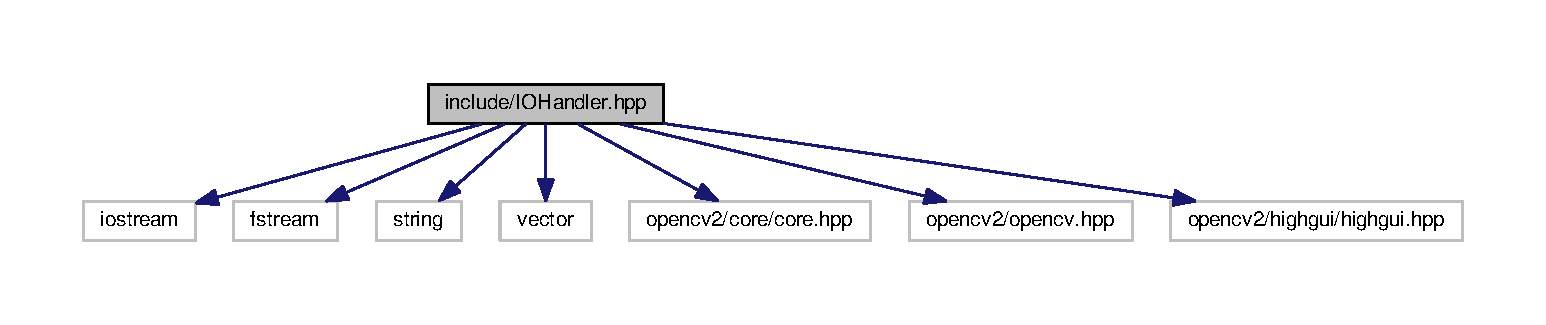
\includegraphics[width=350pt]{IOHandler_8hpp__incl}
\end{center}
\end{figure}
This graph shows which files directly or indirectly include this file\+:\nopagebreak
\begin{figure}[H]
\begin{center}
\leavevmode
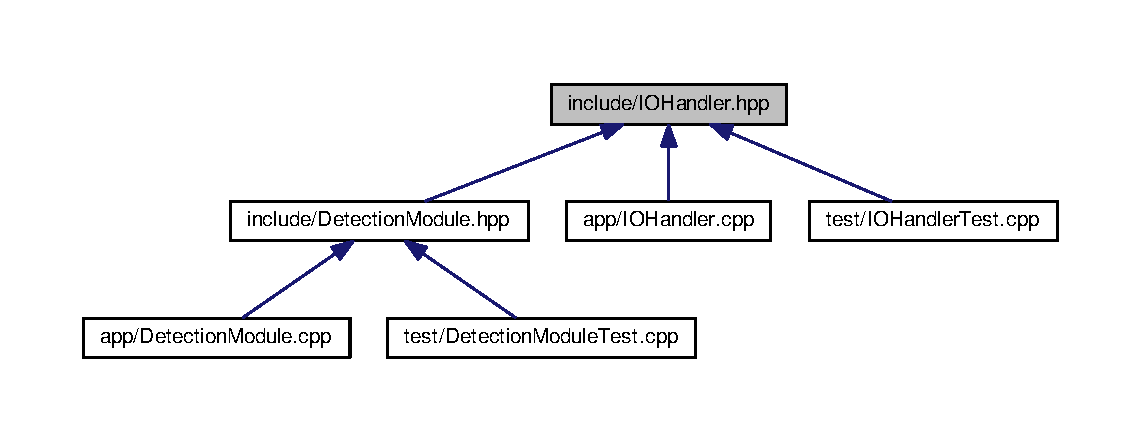
\includegraphics[width=350pt]{IOHandler_8hpp__dep__incl}
\end{center}
\end{figure}
\subsection*{Classes}
\begin{DoxyCompactItemize}
\item 
class \hyperlink{classIOHandler}{I\+O\+Handler}
\begin{DoxyCompactList}\small\item\em Class to manage the input output functionality of the module. \end{DoxyCompactList}\end{DoxyCompactItemize}


\subsection{Detailed Description}
Declares \hyperlink{classIOHandler}{I\+O\+Handler} class. 

\begin{DoxyAuthor}{Author}
Rohan Singh 

Arjun Gupta 
\end{DoxyAuthor}
\begin{DoxyCopyright}{Copyright}
M\+IT License (c) 2019 Rohan Singh, Arjun Gupta 
\end{DoxyCopyright}

\hypertarget{Network_8hpp}{}\section{include/\+Network.hpp File Reference}
\label{Network_8hpp}\index{include/\+Network.\+hpp@{include/\+Network.\+hpp}}


Declares \hyperlink{classNetwork}{Network} class.  


{\ttfamily \#include $<$iostream$>$}\\*
{\ttfamily \#include $<$vector$>$}\\*
{\ttfamily \#include $<$opencv2/dnn.\+hpp$>$}\\*
{\ttfamily \#include $<$opencv2/imgproc.\+hpp$>$}\\*
{\ttfamily \#include $<$opencv2/highgui.\+hpp$>$}\\*
{\ttfamily \#include $<$opencv2/core/core.\+hpp$>$}\\*
{\ttfamily \#include $<$opencv2/opencv.\+hpp$>$}\\*
Include dependency graph for Network.\+hpp\+:\nopagebreak
\begin{figure}[H]
\begin{center}
\leavevmode
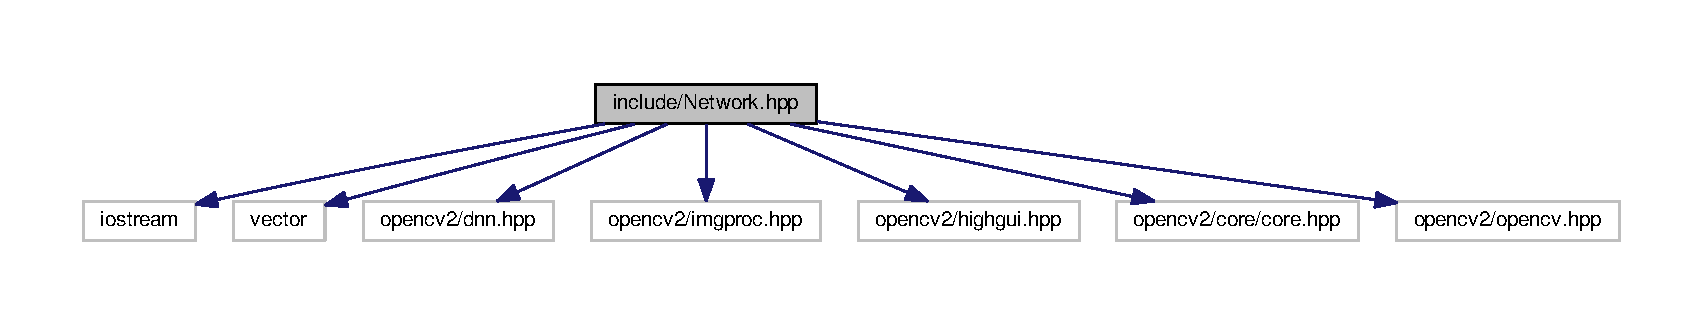
\includegraphics[width=350pt]{Network_8hpp__incl}
\end{center}
\end{figure}
This graph shows which files directly or indirectly include this file\+:\nopagebreak
\begin{figure}[H]
\begin{center}
\leavevmode
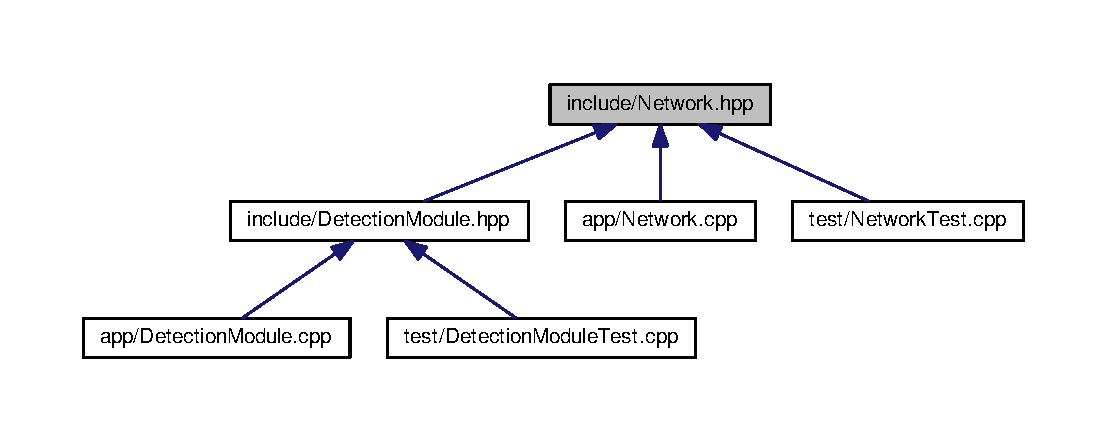
\includegraphics[width=350pt]{Network_8hpp__dep__incl}
\end{center}
\end{figure}
\subsection*{Classes}
\begin{DoxyCompactItemize}
\item 
class \hyperlink{classNetwork}{Network}
\begin{DoxyCompactList}\small\item\em Class for Implementing Neural \hyperlink{classNetwork}{Network} for Human Detection. \end{DoxyCompactList}\end{DoxyCompactItemize}


\subsection{Detailed Description}
Declares \hyperlink{classNetwork}{Network} class. 

\begin{DoxyAuthor}{Author}
Rohan Singh 

Arjun Gupta 
\end{DoxyAuthor}
\begin{DoxyCopyright}{Copyright}
M\+IT License (c) 2019 Rohan Singh, Arjun Gupta 
\end{DoxyCopyright}

\hypertarget{Transformation_8hpp}{}\section{include/\+Transformation.hpp File Reference}
\label{Transformation_8hpp}\index{include/\+Transformation.\+hpp@{include/\+Transformation.\+hpp}}


Declares \hyperlink{classTransformation}{Transformation} class.  


{\ttfamily \#include $<$iostream$>$}\\*
{\ttfamily \#include $<$opencv2/core/core.\+hpp$>$}\\*
{\ttfamily \#include $<$opencv2/core/mat.\+hpp$>$}\\*
{\ttfamily \#include $<$opencv2/opencv.\+hpp$>$}\\*
{\ttfamily \#include $<$opencv2/highgui/highgui.\+hpp$>$}\\*
Include dependency graph for Transformation.\+hpp\+:\nopagebreak
\begin{figure}[H]
\begin{center}
\leavevmode
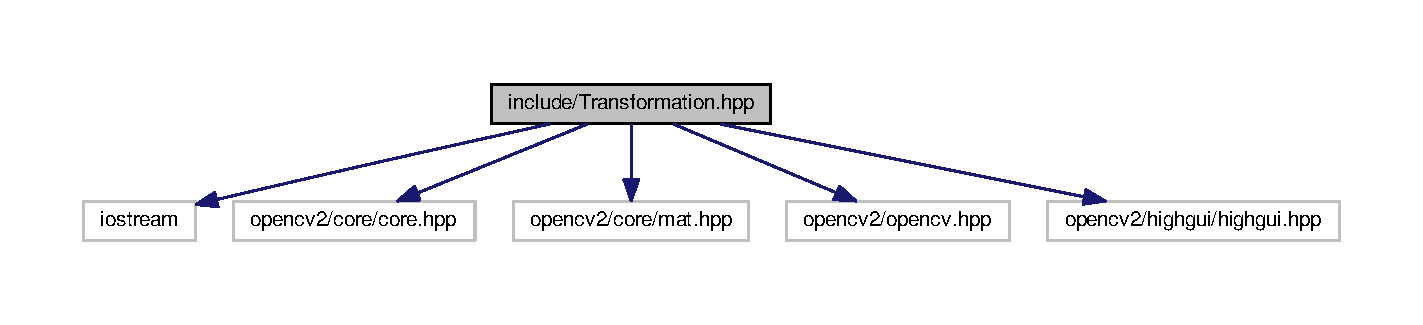
\includegraphics[width=350pt]{Transformation_8hpp__incl}
\end{center}
\end{figure}
This graph shows which files directly or indirectly include this file\+:\nopagebreak
\begin{figure}[H]
\begin{center}
\leavevmode
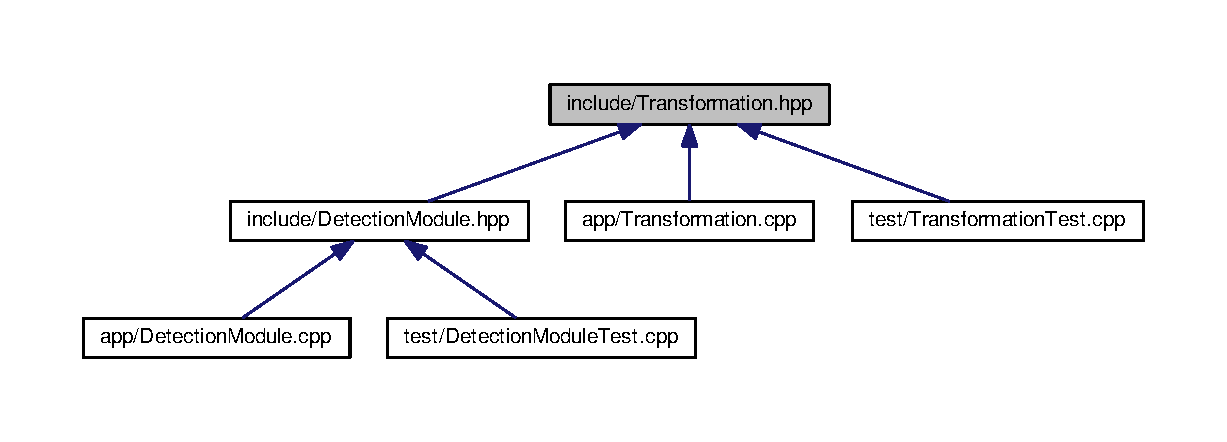
\includegraphics[width=350pt]{Transformation_8hpp__dep__incl}
\end{center}
\end{figure}
\subsection*{Classes}
\begin{DoxyCompactItemize}
\item 
class \hyperlink{classTransformation}{Transformation}
\begin{DoxyCompactList}\small\item\em Class for implementing Frame transformations. \end{DoxyCompactList}\end{DoxyCompactItemize}


\subsection{Detailed Description}
Declares \hyperlink{classTransformation}{Transformation} class. 

\begin{DoxyAuthor}{Author}
Rohan Singh 

Arjun Gupta 
\end{DoxyAuthor}
\begin{DoxyCopyright}{Copyright}
M\+IT License (c) 2019 Rohan Singh, Arjun Gupta 
\end{DoxyCopyright}

\hypertarget{VisionModule_8hpp}{}\section{include/\+Vision\+Module.hpp File Reference}
\label{VisionModule_8hpp}\index{include/\+Vision\+Module.\+hpp@{include/\+Vision\+Module.\+hpp}}


Declares \hyperlink{classVisionModule}{Vision\+Module} base class for \hyperlink{classDetectionModule}{Detection\+Module} class.  


{\ttfamily \#include $<$iostream$>$}\\*
{\ttfamily \#include $<$vector$>$}\\*
{\ttfamily \#include $<$utility$>$}\\*
{\ttfamily \#include $<$opencv2/core/core.\+hpp$>$}\\*
{\ttfamily \#include $<$opencv2/opencv.\+hpp$>$}\\*
{\ttfamily \#include $<$opencv2/highgui/highgui.\+hpp$>$}\\*
Include dependency graph for Vision\+Module.\+hpp\+:\nopagebreak
\begin{figure}[H]
\begin{center}
\leavevmode
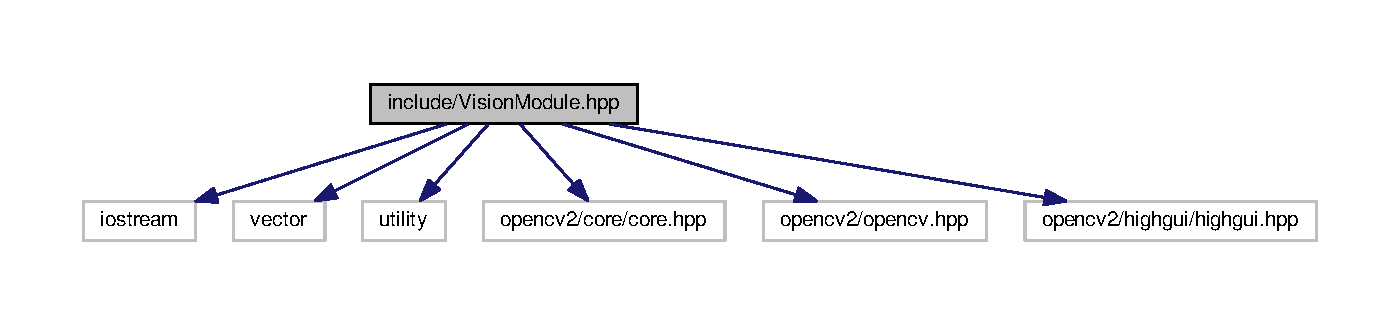
\includegraphics[width=350pt]{VisionModule_8hpp__incl}
\end{center}
\end{figure}
This graph shows which files directly or indirectly include this file\+:\nopagebreak
\begin{figure}[H]
\begin{center}
\leavevmode
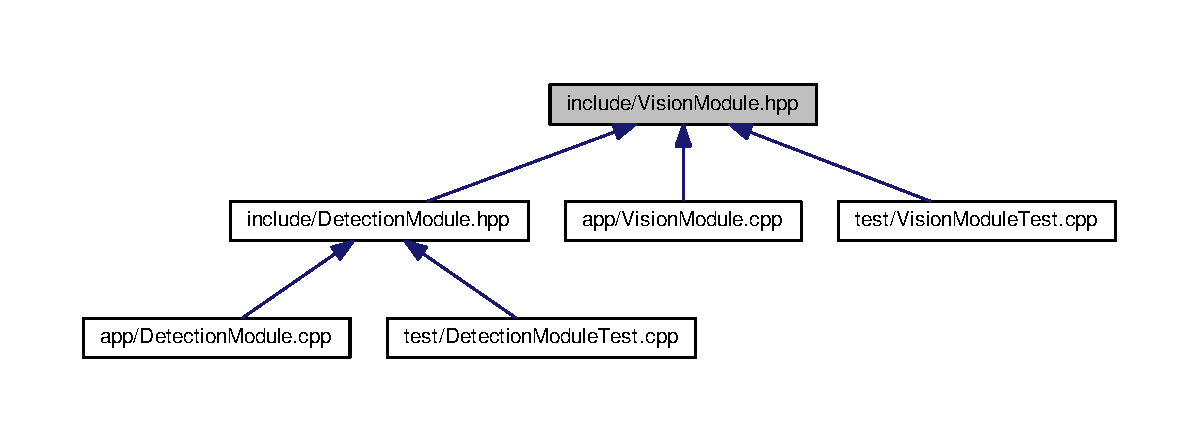
\includegraphics[width=350pt]{VisionModule_8hpp__dep__incl}
\end{center}
\end{figure}
\subsection*{Classes}
\begin{DoxyCompactItemize}
\item 
class \hyperlink{classVisionModule}{Vision\+Module}
\begin{DoxyCompactList}\small\item\em Class for Vision based functionality. \end{DoxyCompactList}\end{DoxyCompactItemize}


\subsection{Detailed Description}
Declares \hyperlink{classVisionModule}{Vision\+Module} base class for \hyperlink{classDetectionModule}{Detection\+Module} class. 

\begin{DoxyAuthor}{Author}
Rohan Singh 

Arjun Gupta 
\end{DoxyAuthor}
\begin{DoxyCopyright}{Copyright}
M\+IT License (c) 2019 Rohan Singh, Arjun Gupta 
\end{DoxyCopyright}

\hypertarget{DetectionModuleTest_8cpp}{}\section{test/\+Detection\+Module\+Test.cpp File Reference}
\label{DetectionModuleTest_8cpp}\index{test/\+Detection\+Module\+Test.\+cpp@{test/\+Detection\+Module\+Test.\+cpp}}


Contains Unit Tests for \hyperlink{classDetectionModule}{Detection\+Module} class.  


{\ttfamily \#include $<$gtest/gtest.\+h$>$}\\*
{\ttfamily \#include $<$Detection\+Module.\+hpp$>$}\\*
Include dependency graph for Detection\+Module\+Test.\+cpp\+:
\nopagebreak
\begin{figure}[H]
\begin{center}
\leavevmode
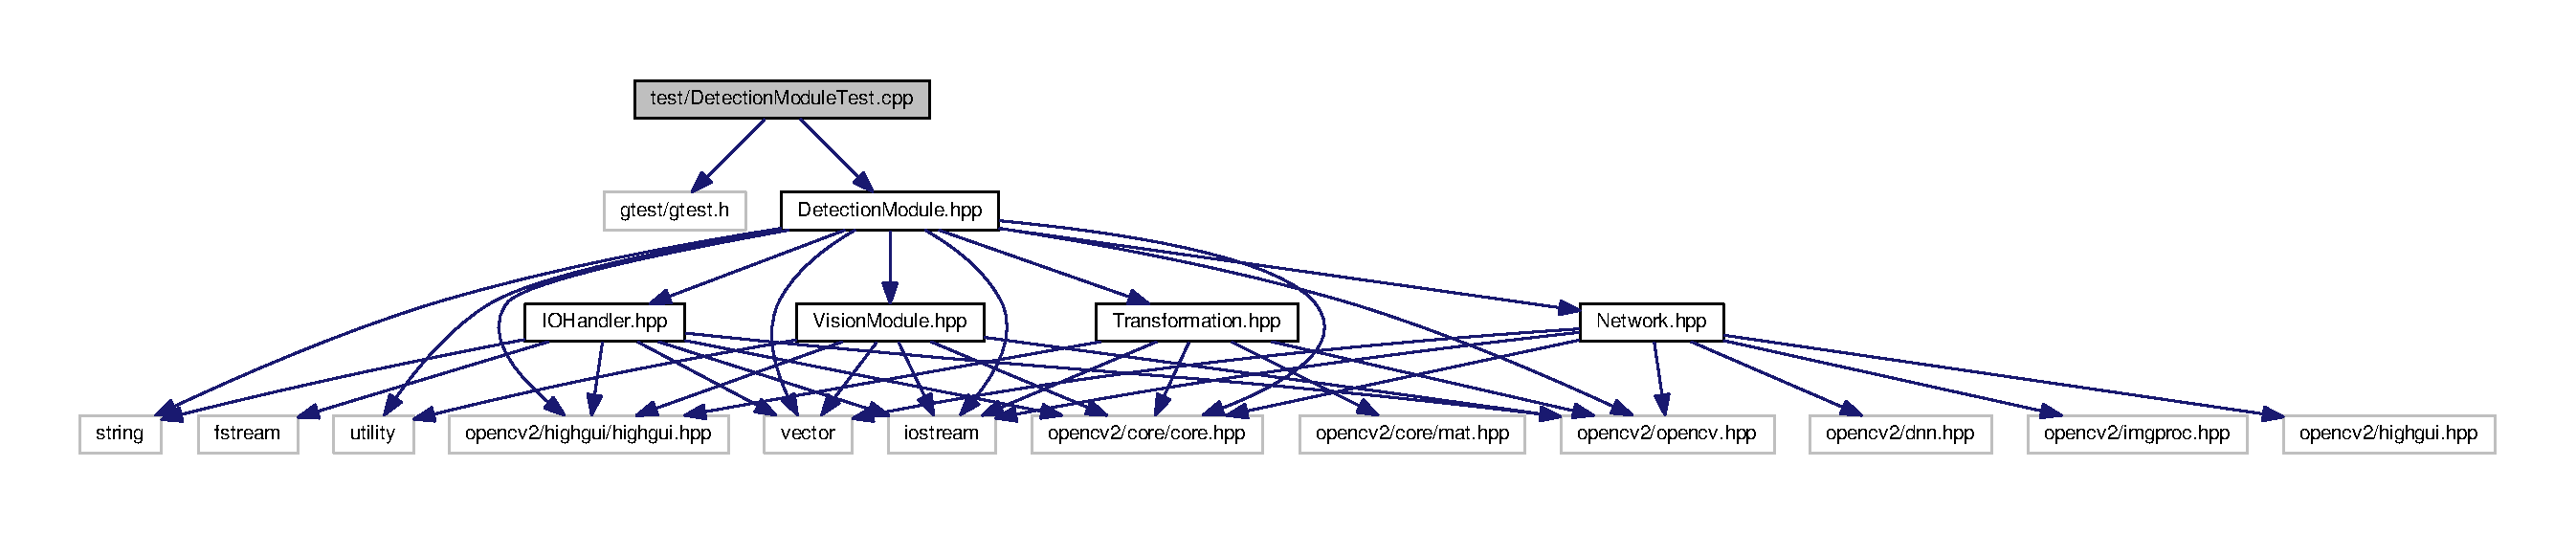
\includegraphics[width=350pt]{DetectionModuleTest_8cpp__incl}
\end{center}
\end{figure}
\subsection*{Functions}
\begin{DoxyCompactItemize}
\item 
\hyperlink{DetectionModuleTest_8cpp_ac8f148a279c04d7b28bc5f1f7728a04e}{T\+E\+ST} (Detection\+Module\+Test, Test\+Get\+Frame)
\begin{DoxyCompactList}\small\item\em Test to check get frame function, that executes main detection functionality. \end{DoxyCompactList}\item 
\hyperlink{DetectionModuleTest_8cpp_a73bdf755e61dc3f82aa7cccdcfd51a38}{T\+E\+ST} (Detection\+Module\+Test, Test\+Pre\+Process\+Image)
\begin{DoxyCompactList}\small\item\em Test to check pre processing steps. \end{DoxyCompactList}\item 
\hyperlink{DetectionModuleTest_8cpp_a11a043f39a0fe2d5f7ef2d424a7d5ea9}{T\+E\+ST} (Detection\+Module\+Test, Test\+Detect\+Objects)
\begin{DoxyCompactList}\small\item\em Test to check network execution. \end{DoxyCompactList}\item 
\hyperlink{DetectionModuleTest_8cpp_a577888da5912d2a9ad35efe62d3ec553}{T\+E\+ST} (Detection\+Module\+Test, Test\+Post\+Process\+Image)
\begin{DoxyCompactList}\small\item\em Test to check post processing steps. \end{DoxyCompactList}\end{DoxyCompactItemize}


\subsection{Detailed Description}
Contains Unit Tests for \hyperlink{classDetectionModule}{Detection\+Module} class. 

\begin{DoxyAuthor}{Author}
Rohan Singh 

Arjun Gupta 
\end{DoxyAuthor}
\begin{DoxyCopyright}{Copyright}
M\+IT License (c) 2019 Rohan Singh, Arjun Gupta 
\end{DoxyCopyright}


\subsection{Function Documentation}
\index{Detection\+Module\+Test.\+cpp@{Detection\+Module\+Test.\+cpp}!T\+E\+ST@{T\+E\+ST}}
\index{T\+E\+ST@{T\+E\+ST}!Detection\+Module\+Test.\+cpp@{Detection\+Module\+Test.\+cpp}}
\subsubsection[{\texorpdfstring{T\+E\+S\+T(\+Detection\+Module\+Test, Test\+Get\+Frame)}{TEST(DetectionModuleTest, TestGetFrame)}}]{\setlength{\rightskip}{0pt plus 5cm}T\+E\+ST (
\begin{DoxyParamCaption}
\item[{Detection\+Module\+Test}]{, }
\item[{Test\+Get\+Frame}]{}
\end{DoxyParamCaption}
)}\hypertarget{DetectionModuleTest_8cpp_ac8f148a279c04d7b28bc5f1f7728a04e}{}\label{DetectionModuleTest_8cpp_ac8f148a279c04d7b28bc5f1f7728a04e}


Test to check get frame function, that executes main detection functionality. 


\begin{DoxyParams}{Parameters}
{\em none} & \\
\hline
\end{DoxyParams}
\begin{DoxyReturn}{Returns}
none 
\end{DoxyReturn}
\index{Detection\+Module\+Test.\+cpp@{Detection\+Module\+Test.\+cpp}!T\+E\+ST@{T\+E\+ST}}
\index{T\+E\+ST@{T\+E\+ST}!Detection\+Module\+Test.\+cpp@{Detection\+Module\+Test.\+cpp}}
\subsubsection[{\texorpdfstring{T\+E\+S\+T(\+Detection\+Module\+Test, Test\+Pre\+Process\+Image)}{TEST(DetectionModuleTest, TestPreProcessImage)}}]{\setlength{\rightskip}{0pt plus 5cm}T\+E\+ST (
\begin{DoxyParamCaption}
\item[{Detection\+Module\+Test}]{, }
\item[{Test\+Pre\+Process\+Image}]{}
\end{DoxyParamCaption}
)}\hypertarget{DetectionModuleTest_8cpp_a73bdf755e61dc3f82aa7cccdcfd51a38}{}\label{DetectionModuleTest_8cpp_a73bdf755e61dc3f82aa7cccdcfd51a38}


Test to check pre processing steps. 


\begin{DoxyParams}{Parameters}
{\em none} & \\
\hline
\end{DoxyParams}
\begin{DoxyReturn}{Returns}
none 
\end{DoxyReturn}
\index{Detection\+Module\+Test.\+cpp@{Detection\+Module\+Test.\+cpp}!T\+E\+ST@{T\+E\+ST}}
\index{T\+E\+ST@{T\+E\+ST}!Detection\+Module\+Test.\+cpp@{Detection\+Module\+Test.\+cpp}}
\subsubsection[{\texorpdfstring{T\+E\+S\+T(\+Detection\+Module\+Test, Test\+Detect\+Objects)}{TEST(DetectionModuleTest, TestDetectObjects)}}]{\setlength{\rightskip}{0pt plus 5cm}T\+E\+ST (
\begin{DoxyParamCaption}
\item[{Detection\+Module\+Test}]{, }
\item[{Test\+Detect\+Objects}]{}
\end{DoxyParamCaption}
)}\hypertarget{DetectionModuleTest_8cpp_a11a043f39a0fe2d5f7ef2d424a7d5ea9}{}\label{DetectionModuleTest_8cpp_a11a043f39a0fe2d5f7ef2d424a7d5ea9}


Test to check network execution. 


\begin{DoxyParams}{Parameters}
{\em none} & \\
\hline
\end{DoxyParams}
\begin{DoxyReturn}{Returns}
none 
\end{DoxyReturn}
\index{Detection\+Module\+Test.\+cpp@{Detection\+Module\+Test.\+cpp}!T\+E\+ST@{T\+E\+ST}}
\index{T\+E\+ST@{T\+E\+ST}!Detection\+Module\+Test.\+cpp@{Detection\+Module\+Test.\+cpp}}
\subsubsection[{\texorpdfstring{T\+E\+S\+T(\+Detection\+Module\+Test, Test\+Post\+Process\+Image)}{TEST(DetectionModuleTest, TestPostProcessImage)}}]{\setlength{\rightskip}{0pt plus 5cm}T\+E\+ST (
\begin{DoxyParamCaption}
\item[{Detection\+Module\+Test}]{, }
\item[{Test\+Post\+Process\+Image}]{}
\end{DoxyParamCaption}
)}\hypertarget{DetectionModuleTest_8cpp_a577888da5912d2a9ad35efe62d3ec553}{}\label{DetectionModuleTest_8cpp_a577888da5912d2a9ad35efe62d3ec553}


Test to check post processing steps. 


\begin{DoxyParams}{Parameters}
{\em none} & \\
\hline
\end{DoxyParams}
\begin{DoxyReturn}{Returns}
none 
\end{DoxyReturn}

\hypertarget{IOHandlerTest_8cpp}{}\section{test/\+I\+O\+Handler\+Test.cpp File Reference}
\label{IOHandlerTest_8cpp}\index{test/\+I\+O\+Handler\+Test.\+cpp@{test/\+I\+O\+Handler\+Test.\+cpp}}


Contains Unit Tests for \hyperlink{classIOHandler}{I\+O\+Handler} class.  


{\ttfamily \#include $<$gtest/gtest.\+h$>$}\\*
{\ttfamily \#include $<$sstream$>$}\\*
{\ttfamily \#include \char`\"{}../include/\+I\+O\+Handler.\+hpp\char`\"{}}\\*
Include dependency graph for I\+O\+Handler\+Test.\+cpp\+:
\nopagebreak
\begin{figure}[H]
\begin{center}
\leavevmode
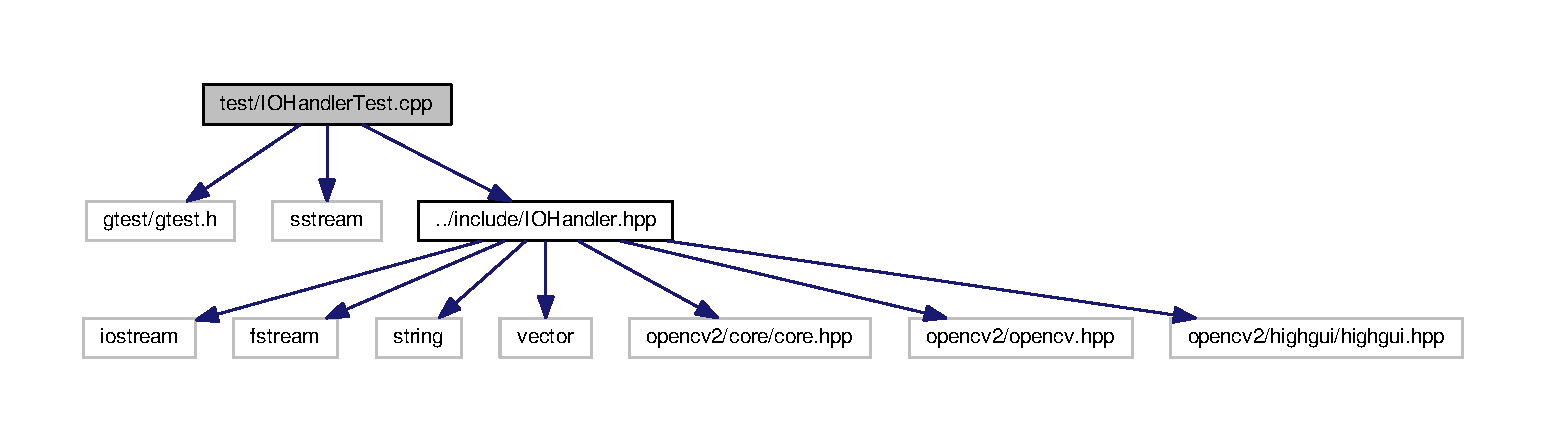
\includegraphics[width=350pt]{IOHandlerTest_8cpp__incl}
\end{center}
\end{figure}
\subsection*{Functions}
\begin{DoxyCompactItemize}
\item 
{\bfseries T\+E\+ST} (\hyperlink{classIOHandler}{I\+O\+Handler}, Test\+Get\+Input\+Choice)\hypertarget{IOHandlerTest_8cpp_a76f7182a356f1b0df3dcf7991609d919}{}\label{IOHandlerTest_8cpp_a76f7182a356f1b0df3dcf7991609d919}

\item 
{\bfseries T\+E\+ST} (\hyperlink{classIOHandler}{I\+O\+Handler}, Test\+Get\+Input\+File\+Path)\hypertarget{IOHandlerTest_8cpp_abb9b5493083dffdd34498379ef4e1c95}{}\label{IOHandlerTest_8cpp_abb9b5493083dffdd34498379ef4e1c95}

\item 
{\bfseries T\+E\+ST} (\hyperlink{classIOHandler}{I\+O\+Handler}, Test\+Get\+Device\+ID)\hypertarget{IOHandlerTest_8cpp_a9d155873e47782345a7736d3cdb2ac9b}{}\label{IOHandlerTest_8cpp_a9d155873e47782345a7736d3cdb2ac9b}

\item 
{\bfseries T\+E\+ST} (\hyperlink{classIOHandler}{I\+O\+Handler}, Test\+Get\+Output\+File\+Path)\hypertarget{IOHandlerTest_8cpp_a4920e52b7910ee39fe5003a581b0e904}{}\label{IOHandlerTest_8cpp_a4920e52b7910ee39fe5003a581b0e904}

\end{DoxyCompactItemize}


\subsection{Detailed Description}
Contains Unit Tests for \hyperlink{classIOHandler}{I\+O\+Handler} class. 

\begin{DoxyAuthor}{Author}
Rohan Singh 

Arjun Gupta 
\end{DoxyAuthor}
\begin{DoxyCopyright}{Copyright}
M\+IT License (c) 2019 Rohan Singh, Arjun Gupta 
\end{DoxyCopyright}

\hypertarget{NetworkTest_8cpp}{}\section{test/\+Network\+Test.cpp File Reference}
\label{NetworkTest_8cpp}\index{test/\+Network\+Test.\+cpp@{test/\+Network\+Test.\+cpp}}


Contains Unit Tests for \hyperlink{classNetwork}{Network} class.  


{\ttfamily \#include $<$gtest/gtest.\+h$>$}\\*
{\ttfamily \#include $<$Network.\+hpp$>$}\\*
Include dependency graph for Network\+Test.\+cpp\+:\nopagebreak
\begin{figure}[H]
\begin{center}
\leavevmode
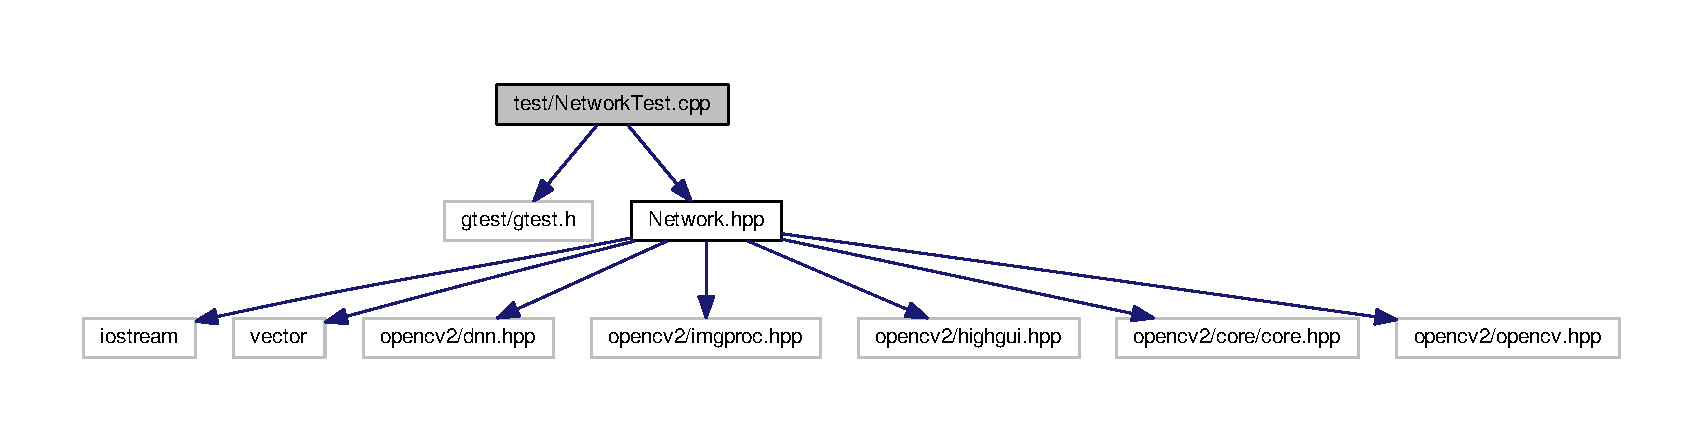
\includegraphics[width=350pt]{NetworkTest_8cpp__incl}
\end{center}
\end{figure}
\subsection*{Functions}
\begin{DoxyCompactItemize}
\item 
\hyperlink{NetworkTest_8cpp_ab10e2660859a3360294bbd9ec328dea7}{T\+E\+ST} (Network\+Test, Test\+Create\+Network\+Input)
\begin{DoxyCompactList}\small\item\em Test to check blob creation. \end{DoxyCompactList}\item 
\hyperlink{NetworkTest_8cpp_a078a884cf7e65d9ad5ec7ee53a55a5cb}{T\+E\+ST} (Network\+Test, Test\+Apply\+Y\+O\+L\+O\+Network)
\begin{DoxyCompactList}\small\item\em Test to check network execution. \end{DoxyCompactList}\end{DoxyCompactItemize}


\subsection{Detailed Description}
Contains Unit Tests for \hyperlink{classNetwork}{Network} class. 

\begin{DoxyAuthor}{Author}
Rohan Singh 

Arjun Gupta 
\end{DoxyAuthor}
\begin{DoxyCopyright}{Copyright}
M\+IT License (c) 2019 Rohan Singh, Arjun Gupta 
\end{DoxyCopyright}


\subsection{Function Documentation}
\index{Network\+Test.\+cpp@{Network\+Test.\+cpp}!T\+E\+ST@{T\+E\+ST}}
\index{T\+E\+ST@{T\+E\+ST}!Network\+Test.\+cpp@{Network\+Test.\+cpp}}
\subsubsection[{\texorpdfstring{T\+E\+S\+T(\+Network\+Test, Test\+Create\+Network\+Input)}{TEST(NetworkTest, TestCreateNetworkInput)}}]{\setlength{\rightskip}{0pt plus 5cm}T\+E\+ST (
\begin{DoxyParamCaption}
\item[{Network\+Test}]{, }
\item[{Test\+Create\+Network\+Input}]{}
\end{DoxyParamCaption}
)}\hypertarget{NetworkTest_8cpp_ab10e2660859a3360294bbd9ec328dea7}{}\label{NetworkTest_8cpp_ab10e2660859a3360294bbd9ec328dea7}


Test to check blob creation. 


\begin{DoxyParams}{Parameters}
{\em none} & \\
\hline
\end{DoxyParams}
\begin{DoxyReturn}{Returns}
none 
\end{DoxyReturn}
\index{Network\+Test.\+cpp@{Network\+Test.\+cpp}!T\+E\+ST@{T\+E\+ST}}
\index{T\+E\+ST@{T\+E\+ST}!Network\+Test.\+cpp@{Network\+Test.\+cpp}}
\subsubsection[{\texorpdfstring{T\+E\+S\+T(\+Network\+Test, Test\+Apply\+Y\+O\+L\+O\+Network)}{TEST(NetworkTest, TestApplyYOLONetwork)}}]{\setlength{\rightskip}{0pt plus 5cm}T\+E\+ST (
\begin{DoxyParamCaption}
\item[{Network\+Test}]{, }
\item[{Test\+Apply\+Y\+O\+L\+O\+Network}]{}
\end{DoxyParamCaption}
)}\hypertarget{NetworkTest_8cpp_a078a884cf7e65d9ad5ec7ee53a55a5cb}{}\label{NetworkTest_8cpp_a078a884cf7e65d9ad5ec7ee53a55a5cb}


Test to check network execution. 


\begin{DoxyParams}{Parameters}
{\em none} & \\
\hline
\end{DoxyParams}
\begin{DoxyReturn}{Returns}
none 
\end{DoxyReturn}

\hypertarget{TransformationTest_8cpp}{}\section{test/\+Transformation\+Test.cpp File Reference}
\label{TransformationTest_8cpp}\index{test/\+Transformation\+Test.\+cpp@{test/\+Transformation\+Test.\+cpp}}


Contains Unit Tests for \hyperlink{classTransformation}{Transformation} class.  


{\ttfamily \#include $<$gtest/gtest.\+h$>$}\\*
{\ttfamily \#include \char`\"{}../include/\+Transformation.\+hpp\char`\"{}}\\*
Include dependency graph for Transformation\+Test.\+cpp\+:\nopagebreak
\begin{figure}[H]
\begin{center}
\leavevmode
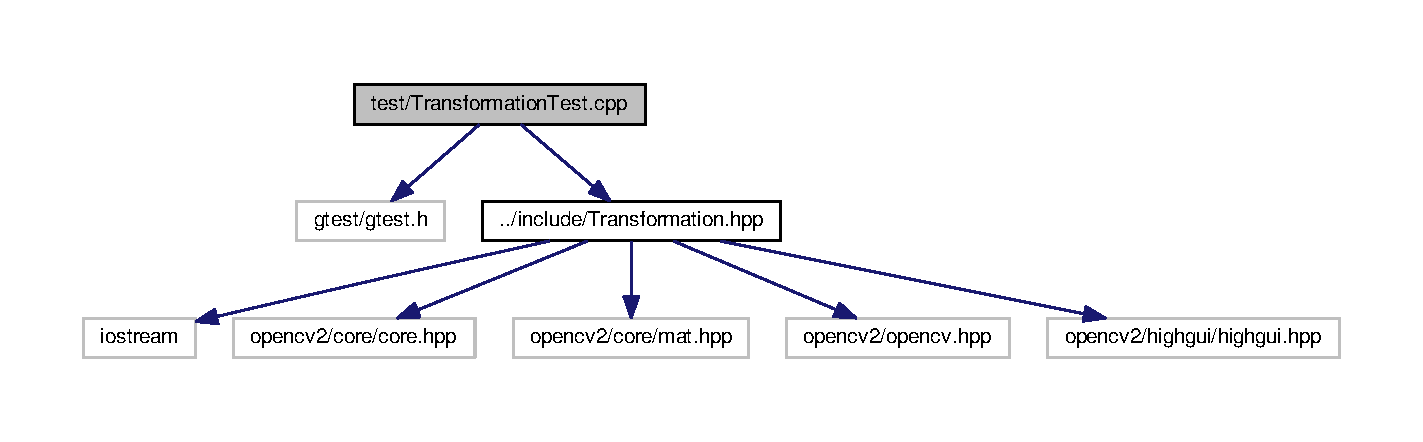
\includegraphics[width=350pt]{TransformationTest_8cpp__incl}
\end{center}
\end{figure}
\subsection*{Functions}
\begin{DoxyCompactItemize}
\item 
\hyperlink{TransformationTest_8cpp_aea111ac3aeb8b1d2034be4403c0d1547}{T\+E\+ST} (Transformation\+Test, Test\+Base\+To\+End)
\begin{DoxyCompactList}\small\item\em Test to check Base frame to End frame transformation. \end{DoxyCompactList}\item 
\hyperlink{TransformationTest_8cpp_aa875cd90705318d0e56a841d124fa7fe}{T\+E\+ST} (Transformation\+Test, Test\+End\+To\+Base)
\begin{DoxyCompactList}\small\item\em Test to check End frame to Base frame transformation. \end{DoxyCompactList}\item 
\hyperlink{TransformationTest_8cpp_affdd1bf49ab6817c6670af326618e280}{T\+E\+ST} (Transformation\+Test, Test\+Image\+To\+Camera)
\begin{DoxyCompactList}\small\item\em Test to check End frame to Base frame transformation. \end{DoxyCompactList}\item 
\hyperlink{TransformationTest_8cpp_a9576161b4838ac429c7b7ea7ef73ae2c}{T\+E\+ST} (Transformation\+Test, Test\+Camera\+To\+Image)
\begin{DoxyCompactList}\small\item\em Test to check End frame to Base frame transformation. \end{DoxyCompactList}\item 
\hyperlink{TransformationTest_8cpp_af7672641649055012daef6d3e84462cd}{T\+E\+ST} (Transformation\+Test, Test\+Get\+Functions)
\begin{DoxyCompactList}\small\item\em Test to check get functions. \end{DoxyCompactList}\end{DoxyCompactItemize}


\subsection{Detailed Description}
Contains Unit Tests for \hyperlink{classTransformation}{Transformation} class. 

\begin{DoxyAuthor}{Author}
Rohan Singh 

Arjun Gupta 
\end{DoxyAuthor}
\begin{DoxyCopyright}{Copyright}
M\+IT License (c) 2019 Rohan Singh, Arjun Gupta 
\end{DoxyCopyright}


\subsection{Function Documentation}
\index{Transformation\+Test.\+cpp@{Transformation\+Test.\+cpp}!T\+E\+ST@{T\+E\+ST}}
\index{T\+E\+ST@{T\+E\+ST}!Transformation\+Test.\+cpp@{Transformation\+Test.\+cpp}}
\subsubsection[{\texorpdfstring{T\+E\+S\+T(\+Transformation\+Test, Test\+Base\+To\+End)}{TEST(TransformationTest, TestBaseToEnd)}}]{\setlength{\rightskip}{0pt plus 5cm}T\+E\+ST (
\begin{DoxyParamCaption}
\item[{Transformation\+Test}]{, }
\item[{Test\+Base\+To\+End}]{}
\end{DoxyParamCaption}
)}\hypertarget{TransformationTest_8cpp_aea111ac3aeb8b1d2034be4403c0d1547}{}\label{TransformationTest_8cpp_aea111ac3aeb8b1d2034be4403c0d1547}


Test to check Base frame to End frame transformation. 


\begin{DoxyParams}{Parameters}
{\em none} & \\
\hline
\end{DoxyParams}
\begin{DoxyReturn}{Returns}
none 
\end{DoxyReturn}
\index{Transformation\+Test.\+cpp@{Transformation\+Test.\+cpp}!T\+E\+ST@{T\+E\+ST}}
\index{T\+E\+ST@{T\+E\+ST}!Transformation\+Test.\+cpp@{Transformation\+Test.\+cpp}}
\subsubsection[{\texorpdfstring{T\+E\+S\+T(\+Transformation\+Test, Test\+End\+To\+Base)}{TEST(TransformationTest, TestEndToBase)}}]{\setlength{\rightskip}{0pt plus 5cm}T\+E\+ST (
\begin{DoxyParamCaption}
\item[{Transformation\+Test}]{, }
\item[{Test\+End\+To\+Base}]{}
\end{DoxyParamCaption}
)}\hypertarget{TransformationTest_8cpp_aa875cd90705318d0e56a841d124fa7fe}{}\label{TransformationTest_8cpp_aa875cd90705318d0e56a841d124fa7fe}


Test to check End frame to Base frame transformation. 


\begin{DoxyParams}{Parameters}
{\em none} & \\
\hline
\end{DoxyParams}
\begin{DoxyReturn}{Returns}
none 
\end{DoxyReturn}
\index{Transformation\+Test.\+cpp@{Transformation\+Test.\+cpp}!T\+E\+ST@{T\+E\+ST}}
\index{T\+E\+ST@{T\+E\+ST}!Transformation\+Test.\+cpp@{Transformation\+Test.\+cpp}}
\subsubsection[{\texorpdfstring{T\+E\+S\+T(\+Transformation\+Test, Test\+Image\+To\+Camera)}{TEST(TransformationTest, TestImageToCamera)}}]{\setlength{\rightskip}{0pt plus 5cm}T\+E\+ST (
\begin{DoxyParamCaption}
\item[{Transformation\+Test}]{, }
\item[{Test\+Image\+To\+Camera}]{}
\end{DoxyParamCaption}
)}\hypertarget{TransformationTest_8cpp_affdd1bf49ab6817c6670af326618e280}{}\label{TransformationTest_8cpp_affdd1bf49ab6817c6670af326618e280}


Test to check End frame to Base frame transformation. 


\begin{DoxyParams}{Parameters}
{\em none} & \\
\hline
\end{DoxyParams}
\begin{DoxyReturn}{Returns}
none 
\end{DoxyReturn}
\index{Transformation\+Test.\+cpp@{Transformation\+Test.\+cpp}!T\+E\+ST@{T\+E\+ST}}
\index{T\+E\+ST@{T\+E\+ST}!Transformation\+Test.\+cpp@{Transformation\+Test.\+cpp}}
\subsubsection[{\texorpdfstring{T\+E\+S\+T(\+Transformation\+Test, Test\+Camera\+To\+Image)}{TEST(TransformationTest, TestCameraToImage)}}]{\setlength{\rightskip}{0pt plus 5cm}T\+E\+ST (
\begin{DoxyParamCaption}
\item[{Transformation\+Test}]{, }
\item[{Test\+Camera\+To\+Image}]{}
\end{DoxyParamCaption}
)}\hypertarget{TransformationTest_8cpp_a9576161b4838ac429c7b7ea7ef73ae2c}{}\label{TransformationTest_8cpp_a9576161b4838ac429c7b7ea7ef73ae2c}


Test to check End frame to Base frame transformation. 


\begin{DoxyParams}{Parameters}
{\em none} & \\
\hline
\end{DoxyParams}
\begin{DoxyReturn}{Returns}
none 
\end{DoxyReturn}
\index{Transformation\+Test.\+cpp@{Transformation\+Test.\+cpp}!T\+E\+ST@{T\+E\+ST}}
\index{T\+E\+ST@{T\+E\+ST}!Transformation\+Test.\+cpp@{Transformation\+Test.\+cpp}}
\subsubsection[{\texorpdfstring{T\+E\+S\+T(\+Transformation\+Test, Test\+Get\+Functions)}{TEST(TransformationTest, TestGetFunctions)}}]{\setlength{\rightskip}{0pt plus 5cm}T\+E\+ST (
\begin{DoxyParamCaption}
\item[{Transformation\+Test}]{, }
\item[{Test\+Get\+Functions}]{}
\end{DoxyParamCaption}
)}\hypertarget{TransformationTest_8cpp_af7672641649055012daef6d3e84462cd}{}\label{TransformationTest_8cpp_af7672641649055012daef6d3e84462cd}


Test to check get functions. 


\begin{DoxyParams}{Parameters}
{\em none} & \\
\hline
\end{DoxyParams}
\begin{DoxyReturn}{Returns}
none 
\end{DoxyReturn}

\hypertarget{VisionModuleTest_8cpp}{}\section{test/\+Vision\+Module\+Test.cpp File Reference}
\label{VisionModuleTest_8cpp}\index{test/\+Vision\+Module\+Test.\+cpp@{test/\+Vision\+Module\+Test.\+cpp}}


Contains Unit Tests for \hyperlink{classVisionModule}{Vision\+Module} class.  


{\ttfamily \#include $<$gtest/gtest.\+h$>$}\\*
{\ttfamily \#include \char`\"{}../include/\+Vision\+Module.\+hpp\char`\"{}}\\*
Include dependency graph for Vision\+Module\+Test.\+cpp\+:\nopagebreak
\begin{figure}[H]
\begin{center}
\leavevmode
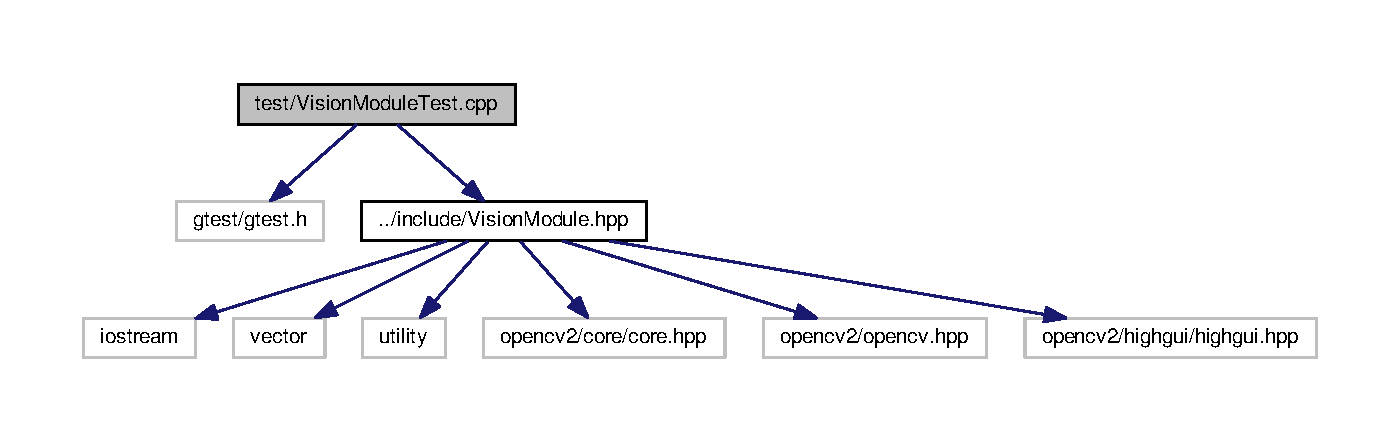
\includegraphics[width=350pt]{VisionModuleTest_8cpp__incl}
\end{center}
\end{figure}
\subsection*{Functions}
\begin{DoxyCompactItemize}
\item 
\hyperlink{VisionModuleTest_8cpp_a0039d57c97c85304951fc70dc3940d0e}{T\+E\+ST} (Vision\+Module\+Test, Test\+Apply\+Gaussian\+Filter)
\begin{DoxyCompactList}\small\item\em Test to check gaussian filter function. \end{DoxyCompactList}\item 
\hyperlink{VisionModuleTest_8cpp_aff95870669b793fcbcd31f4bc8cef129}{T\+E\+ST} (Vision\+Module\+Test, Test\+Apply\+Mean\+Filter)
\begin{DoxyCompactList}\small\item\em Test to check mean filter function. \end{DoxyCompactList}\item 
\hyperlink{VisionModuleTest_8cpp_a42b09d676d5e1b5e9b67e726e10b4b1f}{T\+E\+ST} (Vision\+Module\+Test, Test\+Apply\+Median\+Filter)
\begin{DoxyCompactList}\small\item\em Test to check median filter function. \end{DoxyCompactList}\item 
\hyperlink{VisionModuleTest_8cpp_ab78f294d393c57ab235d32ce6f9cb0b3}{T\+E\+ST} (Vision\+Module\+Test, Test\+Reshape)
\begin{DoxyCompactList}\small\item\em Test to check image reshape function. \end{DoxyCompactList}\item 
\hyperlink{VisionModuleTest_8cpp_abaf2671cebadcd966f404c8caafd00b5}{T\+E\+ST} (Vision\+Module\+Test, Test\+Non\+Maximal\+Suppression)
\begin{DoxyCompactList}\small\item\em Test to check non-\/maximal suppression algorithm. \end{DoxyCompactList}\end{DoxyCompactItemize}


\subsection{Detailed Description}
Contains Unit Tests for \hyperlink{classVisionModule}{Vision\+Module} class. 

\begin{DoxyAuthor}{Author}
Rohan Singh 

Arjun Gupta 
\end{DoxyAuthor}
\begin{DoxyCopyright}{Copyright}
M\+IT License (c) 2019 Rohan Singh, Arjun Gupta 
\end{DoxyCopyright}


\subsection{Function Documentation}
\index{Vision\+Module\+Test.\+cpp@{Vision\+Module\+Test.\+cpp}!T\+E\+ST@{T\+E\+ST}}
\index{T\+E\+ST@{T\+E\+ST}!Vision\+Module\+Test.\+cpp@{Vision\+Module\+Test.\+cpp}}
\subsubsection[{\texorpdfstring{T\+E\+S\+T(\+Vision\+Module\+Test, Test\+Apply\+Gaussian\+Filter)}{TEST(VisionModuleTest, TestApplyGaussianFilter)}}]{\setlength{\rightskip}{0pt plus 5cm}T\+E\+ST (
\begin{DoxyParamCaption}
\item[{Vision\+Module\+Test}]{, }
\item[{Test\+Apply\+Gaussian\+Filter}]{}
\end{DoxyParamCaption}
)}\hypertarget{VisionModuleTest_8cpp_a0039d57c97c85304951fc70dc3940d0e}{}\label{VisionModuleTest_8cpp_a0039d57c97c85304951fc70dc3940d0e}


Test to check gaussian filter function. 


\begin{DoxyParams}{Parameters}
{\em none} & \\
\hline
\end{DoxyParams}
\begin{DoxyReturn}{Returns}
none 
\end{DoxyReturn}
\index{Vision\+Module\+Test.\+cpp@{Vision\+Module\+Test.\+cpp}!T\+E\+ST@{T\+E\+ST}}
\index{T\+E\+ST@{T\+E\+ST}!Vision\+Module\+Test.\+cpp@{Vision\+Module\+Test.\+cpp}}
\subsubsection[{\texorpdfstring{T\+E\+S\+T(\+Vision\+Module\+Test, Test\+Apply\+Mean\+Filter)}{TEST(VisionModuleTest, TestApplyMeanFilter)}}]{\setlength{\rightskip}{0pt plus 5cm}T\+E\+ST (
\begin{DoxyParamCaption}
\item[{Vision\+Module\+Test}]{, }
\item[{Test\+Apply\+Mean\+Filter}]{}
\end{DoxyParamCaption}
)}\hypertarget{VisionModuleTest_8cpp_aff95870669b793fcbcd31f4bc8cef129}{}\label{VisionModuleTest_8cpp_aff95870669b793fcbcd31f4bc8cef129}


Test to check mean filter function. 


\begin{DoxyParams}{Parameters}
{\em none} & \\
\hline
\end{DoxyParams}
\begin{DoxyReturn}{Returns}
none 
\end{DoxyReturn}
\index{Vision\+Module\+Test.\+cpp@{Vision\+Module\+Test.\+cpp}!T\+E\+ST@{T\+E\+ST}}
\index{T\+E\+ST@{T\+E\+ST}!Vision\+Module\+Test.\+cpp@{Vision\+Module\+Test.\+cpp}}
\subsubsection[{\texorpdfstring{T\+E\+S\+T(\+Vision\+Module\+Test, Test\+Apply\+Median\+Filter)}{TEST(VisionModuleTest, TestApplyMedianFilter)}}]{\setlength{\rightskip}{0pt plus 5cm}T\+E\+ST (
\begin{DoxyParamCaption}
\item[{Vision\+Module\+Test}]{, }
\item[{Test\+Apply\+Median\+Filter}]{}
\end{DoxyParamCaption}
)}\hypertarget{VisionModuleTest_8cpp_a42b09d676d5e1b5e9b67e726e10b4b1f}{}\label{VisionModuleTest_8cpp_a42b09d676d5e1b5e9b67e726e10b4b1f}


Test to check median filter function. 


\begin{DoxyParams}{Parameters}
{\em none} & \\
\hline
\end{DoxyParams}
\begin{DoxyReturn}{Returns}
none 
\end{DoxyReturn}
\index{Vision\+Module\+Test.\+cpp@{Vision\+Module\+Test.\+cpp}!T\+E\+ST@{T\+E\+ST}}
\index{T\+E\+ST@{T\+E\+ST}!Vision\+Module\+Test.\+cpp@{Vision\+Module\+Test.\+cpp}}
\subsubsection[{\texorpdfstring{T\+E\+S\+T(\+Vision\+Module\+Test, Test\+Reshape)}{TEST(VisionModuleTest, TestReshape)}}]{\setlength{\rightskip}{0pt plus 5cm}T\+E\+ST (
\begin{DoxyParamCaption}
\item[{Vision\+Module\+Test}]{, }
\item[{Test\+Reshape}]{}
\end{DoxyParamCaption}
)}\hypertarget{VisionModuleTest_8cpp_ab78f294d393c57ab235d32ce6f9cb0b3}{}\label{VisionModuleTest_8cpp_ab78f294d393c57ab235d32ce6f9cb0b3}


Test to check image reshape function. 


\begin{DoxyParams}{Parameters}
{\em none} & \\
\hline
\end{DoxyParams}
\begin{DoxyReturn}{Returns}
none 
\end{DoxyReturn}
\index{Vision\+Module\+Test.\+cpp@{Vision\+Module\+Test.\+cpp}!T\+E\+ST@{T\+E\+ST}}
\index{T\+E\+ST@{T\+E\+ST}!Vision\+Module\+Test.\+cpp@{Vision\+Module\+Test.\+cpp}}
\subsubsection[{\texorpdfstring{T\+E\+S\+T(\+Vision\+Module\+Test, Test\+Non\+Maximal\+Suppression)}{TEST(VisionModuleTest, TestNonMaximalSuppression)}}]{\setlength{\rightskip}{0pt plus 5cm}T\+E\+ST (
\begin{DoxyParamCaption}
\item[{Vision\+Module\+Test}]{, }
\item[{Test\+Non\+Maximal\+Suppression}]{}
\end{DoxyParamCaption}
)}\hypertarget{VisionModuleTest_8cpp_abaf2671cebadcd966f404c8caafd00b5}{}\label{VisionModuleTest_8cpp_abaf2671cebadcd966f404c8caafd00b5}


Test to check non-\/maximal suppression algorithm. 


\begin{DoxyParams}{Parameters}
{\em none} & \\
\hline
\end{DoxyParams}
\begin{DoxyReturn}{Returns}
none 
\end{DoxyReturn}

%--- End generated contents ---

% Index
\backmatter
\newpage
\phantomsection
\clearemptydoublepage
\addcontentsline{toc}{chapter}{Index}
\printindex

\end{document}
